%%%%%%%%%1%%%%%%%%%2%%%%%%%%%3%%%%%%%%%4%%%%%%%%%5%%%%%%%%%6
% Beamer Header
%%%%%%%%%1%%%%%%%%%2%%%%%%%%%3%%%%%%%%%4%%%%%%%%%5%%%%%%%%%6

\documentclass[compress,english]{beamer}
\usetheme{sthlm}

% Basic beamer packages
\usepackage{booktabs}
\usepackage{datetime}
\usepackage{graphicx}
\usepackage{multicol}
\usepackage{pgfplots}
\usepackage{ragged2e}
\usepackage{tabularx}
\usepackage{tikz}
\usepackage{wasysym}

\pgfplotsset{compat=1.8}

\usepackage[utf8]{inputenc}
\usepackage[T1]{fontenc}
%\usepackage{newpxtext,newpxmath}

% tikz
\usepackage{tikz}
\usetikzlibrary{patterns,backgrounds,mindmap}

% additional packages
\usepackage{listings}
\usepackage{units}
\usepackage{babel}
\usepackage{sansmath}
%\usepackage{chemfig}
%\usepackage{mhchem}

\makeatother
%%%%%%%%%1%%%%%%%%%2%%%%%%%%%3%%%%%%%%%4%%%%%%%%%5%%%%%%%%%6
% Graphics Path
%%%%%%%%%1%%%%%%%%%2%%%%%%%%%3%%%%%%%%%4%%%%%%%%%5%%%%%%%%%6

\graphicspath{
	{images/}
	{../images/}
	{../../images/}
}

%%%%%%%%%1%%%%%%%%%2%%%%%%%%%3%%%%%%%%%4%%%%%%%%%5%%%%%%%%%6
% Footnote rule
%%%%%%%%%1%%%%%%%%%2%%%%%%%%%3%%%%%%%%%4%%%%%%%%%5%%%%%%%%%6

\renewcommand{\footnoterule}{%
}
  
%%%%%%%%%1%%%%%%%%%2%%%%%%%%%3%%%%%%%%%4%%%%%%%%%5%%%%%%%%%6
% Default Background Image
%%%%%%%%%1%%%%%%%%%2%%%%%%%%%3%%%%%%%%%4%%%%%%%%%5%%%%%%%%%6

\usebackgroundtemplate%
	{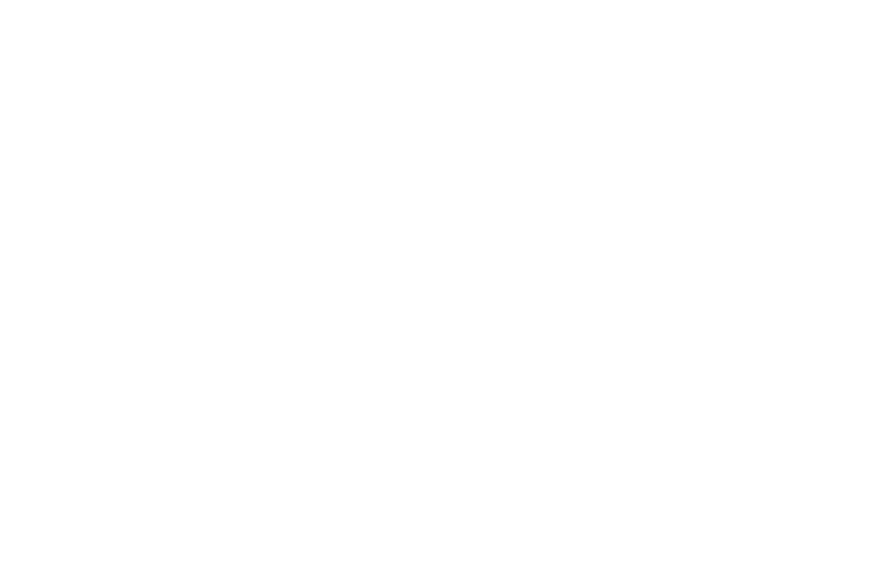
\includegraphics[width=\paperwidth,height=\paperheight]{background.png}}

%%%%%%%%%1%%%%%%%%%2%%%%%%%%%3%%%%%%%%%4%%%%%%%%%5%%%%%%%%%6
% Presentation Information
%%%%%%%%%1%%%%%%%%%2%%%%%%%%%3%%%%%%%%%4%%%%%%%%%5%%%%%%%%%6

\title{\large Predictive Control and Estimation of Lake Levels and Stream Flows for the Adaptive Management of Complex Natural Watersheds and Ecosystems.}
\subtitle{Part 1. Estimation.\\
Part 2. Economic Model Predictive Control.}

\author{Jeffrey Kantor }
\institute{University of Notre Dame \\ Github: \href{http://jckantor.github.io/Rainy-Lake-Hydrology/}{http://jckantor.github.io/Rainy-Lake-Hydrology/}}
\date{2017 AIChE Annual Meeting \\ 
      October 31, 2017}

\begin{document}

%%%%%%%%%1%%%%%%%%%2%%%%%%%%%3%%%%%%%%%4%%%%%%%%%5%%%%%%%%%6
% Title Page
%%%%%%%%%1%%%%%%%%%2%%%%%%%%%3%%%%%%%%%4%%%%%%%%%5%%%%%%%%%6

\setbeamercolor{title}{fg=white}
\setbeamercolor{subtitle}{fg=white}
\setbeamercolor{date}{fg=white}
\setbeamercolor{author}{fg=white}
\setbeamercolor{institute}{fg=white}

\setbeamerfont{title}{series=\bfseries}

{\usebackgroundtemplate%
	{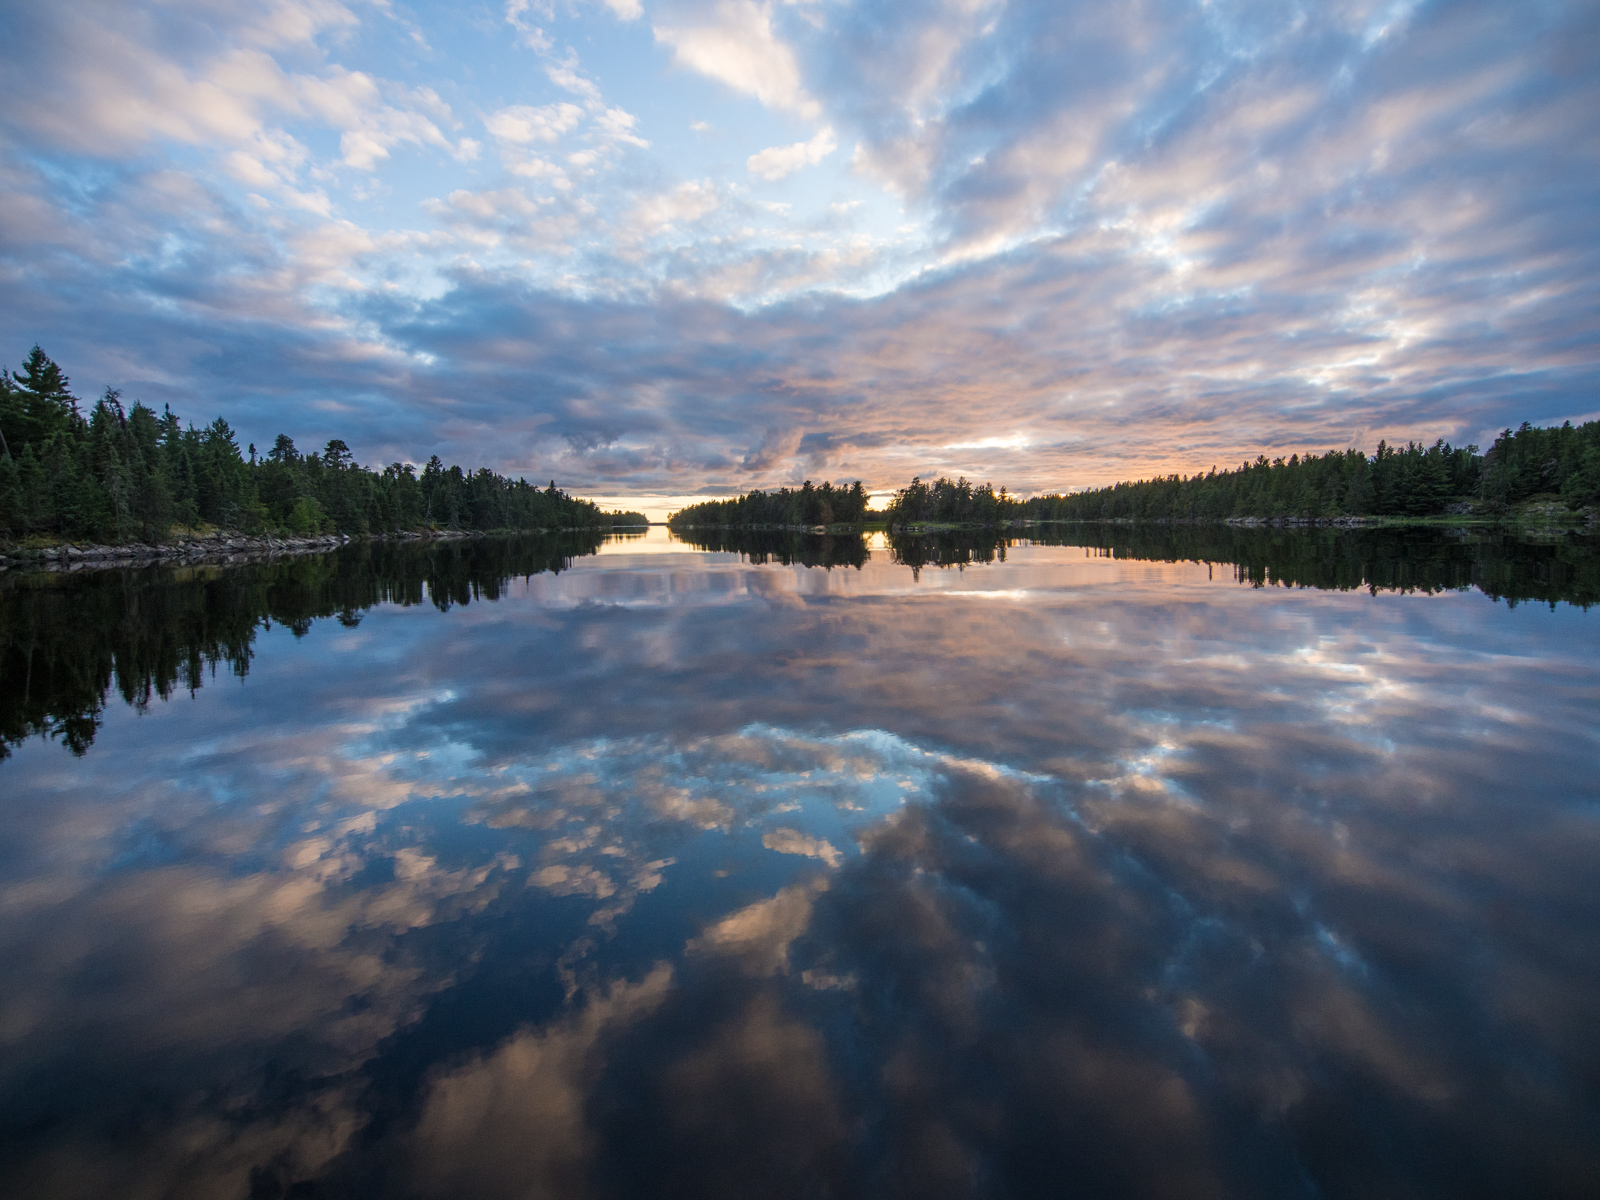
\includegraphics[height=\paperheight]{20150804_202405.jpg}}
\begin{frame}[plain]
\titlepage
\end{frame}
}

%%%%%%%%%1%%%%%%%%%2%%%%%%%%%3%%%%%%%%%4%%%%%%%%%5%%%%%%%%%6
% Table of Contents
%%%%%%%%%1%%%%%%%%%2%%%%%%%%%3%%%%%%%%%4%%%%%%%%%5%%%%%%%%%6
\begin{frame}{Overview}
% For longer presentations hideallsubsections
\tableofcontents[hideallsubsections]
\end{frame}

%%%%%%%%%1%%%%%%%%%2%%%%%%%%%3%%%%%%%%%4%%%%%%%%%5%%%%%%%%%6
% Section
%%%%%%%%%1%%%%%%%%%2%%%%%%%%%3%%%%%%%%%4%%%%%%%%%5%%%%%%%%%6
{\usebackgroundtemplate%
	{
\includegraphics[height=\paperheight]{background_grey.png}}
\section{Overview}
}

%%%%%%%%%1%%%%%%%%%2%%%%%%%%%3%%%%%%%%%4%%%%%%%%%5%%%%%%%%%6
\begin{frame}{Overall Water Risk - WRI 2015}

\begin{center}
\includegraphicscopyright[width=0.9\paperwidth]{aqueduct_global_maps_21.png}{Source: World Resources Institute, Ver 2.1, 2015.}
\end{center}
This map summarizes water risks associated with scarcity.
\end{frame}

%%%%%%%%%1%%%%%%%%%2%%%%%%%%%3%%%%%%%%%4%%%%%%%%%5%%%%%%%%%6
\begin{frame}{Transboundary Aquifers of the World}

\begin{center}
\includegraphicscopyright[width=0.75\paperwidth]{TBA-Map-colour.jpg}{Source: The International Law of Transboundary Groundwater Resources,  2017.}
\end{center}
\begin{itemize}
\item Ubiquitous: 450 shared aquifers
\item Strategic: 50\% of global domestic needs, 40\% of agriculture.
\item Legal Vacuum: No global conventions
\item Information Scarcity: Sovereign states with strong self-interests
\end{itemize}

\end{frame}

%%%%%%%%%1%%%%%%%%%2%%%%%%%%%3%%%%%%%%%4%%%%%%%%%5%%%%%%%%%6
\begin{frame}{Transboundary Waters of Canada and the US}

\begin{center}
\includegraphicscopyright[width=0.8\paperwidth]{CAN-US-Boundary-Waters.jpg}{Source: Canadian Encylopedia.}
\end{center}

US and Canada share 8,000 km border that is 45\% water with over 300 lakes and streams.

Boundary Waters Treaty of 1909 established the International Joint Commission to govern transboundary water.
\end{frame}

%%%%%%%%%1%%%%%%%%%2%%%%%%%%%3%%%%%%%%%4%%%%%%%%%5%%%%%%%%%6
\begin{frame}{Rainy River Drainage Basin}

\begin{center}
\includegraphicscopyright[width=0.7\paperwidth]{75242923}{Source: International Rainy Lake Board of Control (now IRLWWB)}
\end{center}
50,000 km$^2$ watershed including pristine wilderness areas.

\end{frame}

%%%%%%%%%1%%%%%%%%%2%%%%%%%%%3%%%%%%%%%4%%%%%%%%%5%%%%%%%%%6
\begin{frame}{Canadian Shield - Lakes > 100 km$^2$}

\begin{columns}
\begin{column}{0.6\textwidth}
\begin{center}
\includegraphicscopyright[height=0.6\paperheight]{69640d77-4187-463e-9293-9d3a0b93364f.jpg}{Source: Canadian Encylopedia.}
\end{center}
\end{column}
\begin{column}{0.4\textwidth}
\begin{center}
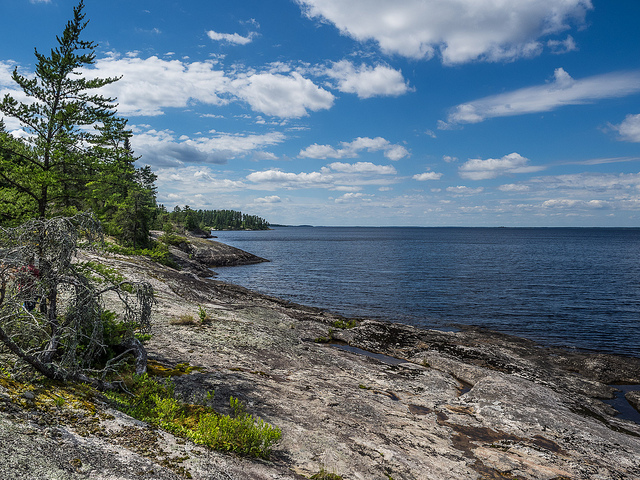
\includegraphics[width=\textwidth]{27843082153_d07e65b8ce_z.jpg}

\includegraphicscopyright[width=\textwidth]{18533803326_aba91e1a90_z.jpg}{Source: Jeff Kantor.}
\end{center}
\end{column}
\end{columns}

The Canadian shield is the geological core of the North American continent (the North American Craton) characterized by exposed Precambrian igneous and high-grade metamorphic rocks.
\end{frame}

%%%%%%%%%1%%%%%%%%%2%%%%%%%%%3%%%%%%%%%4%%%%%%%%%5%%%%%%%%%6
\begin{frame}{Major Control Points}

\begin{center}
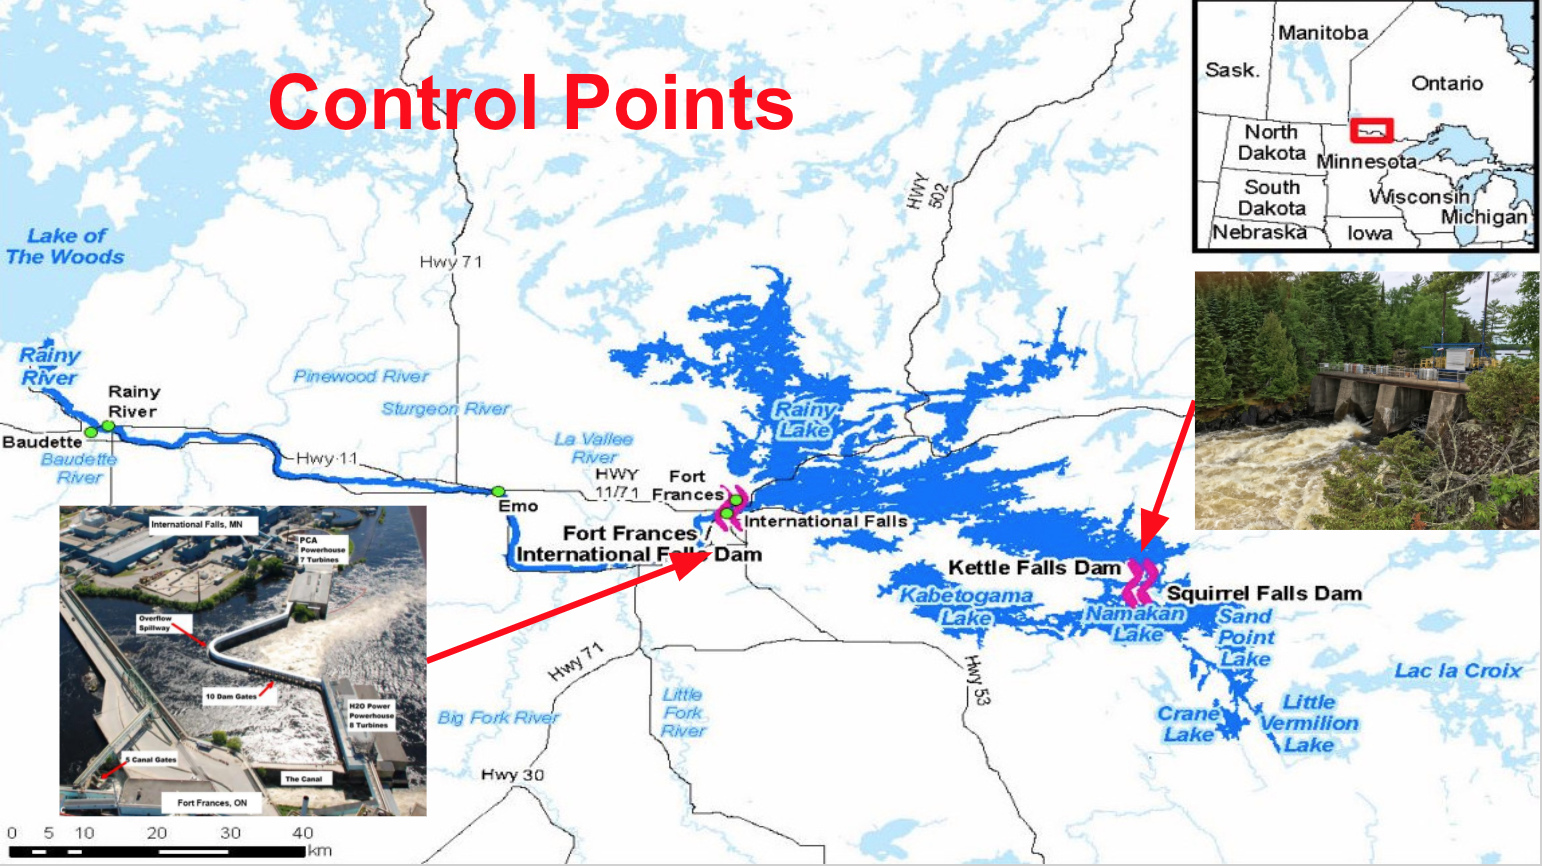
\includegraphics[width=0.9\paperwidth]{ControlPoints}
\end{center}

\end{frame}

%%%%%%%%%1%%%%%%%%%2%%%%%%%%%3%%%%%%%%%4%%%%%%%%%5%%%%%%%%%6
{\usebackgroundtemplate%
	{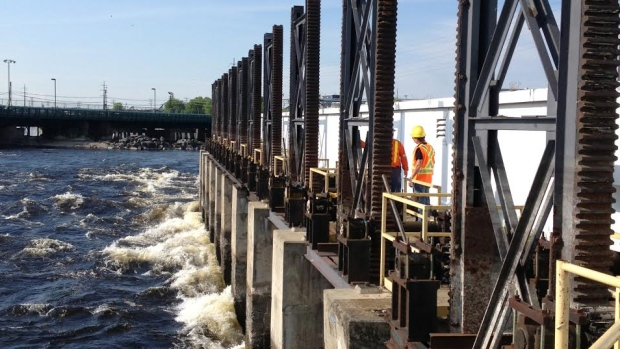
\includegraphics[height=\paperheight]{fort-frances-dam.jpg}}
\begin{frame}{Dam at International Falls, MN/Fort Frances, Ont}	
\end{frame}
}

%%%%%%%%%1%%%%%%%%%2%%%%%%%%%3%%%%%%%%%4%%%%%%%%%5%%%%%%%%%6
\begin{frame}{Dam at Kettle/Squirrel Falls}

\begin{center}
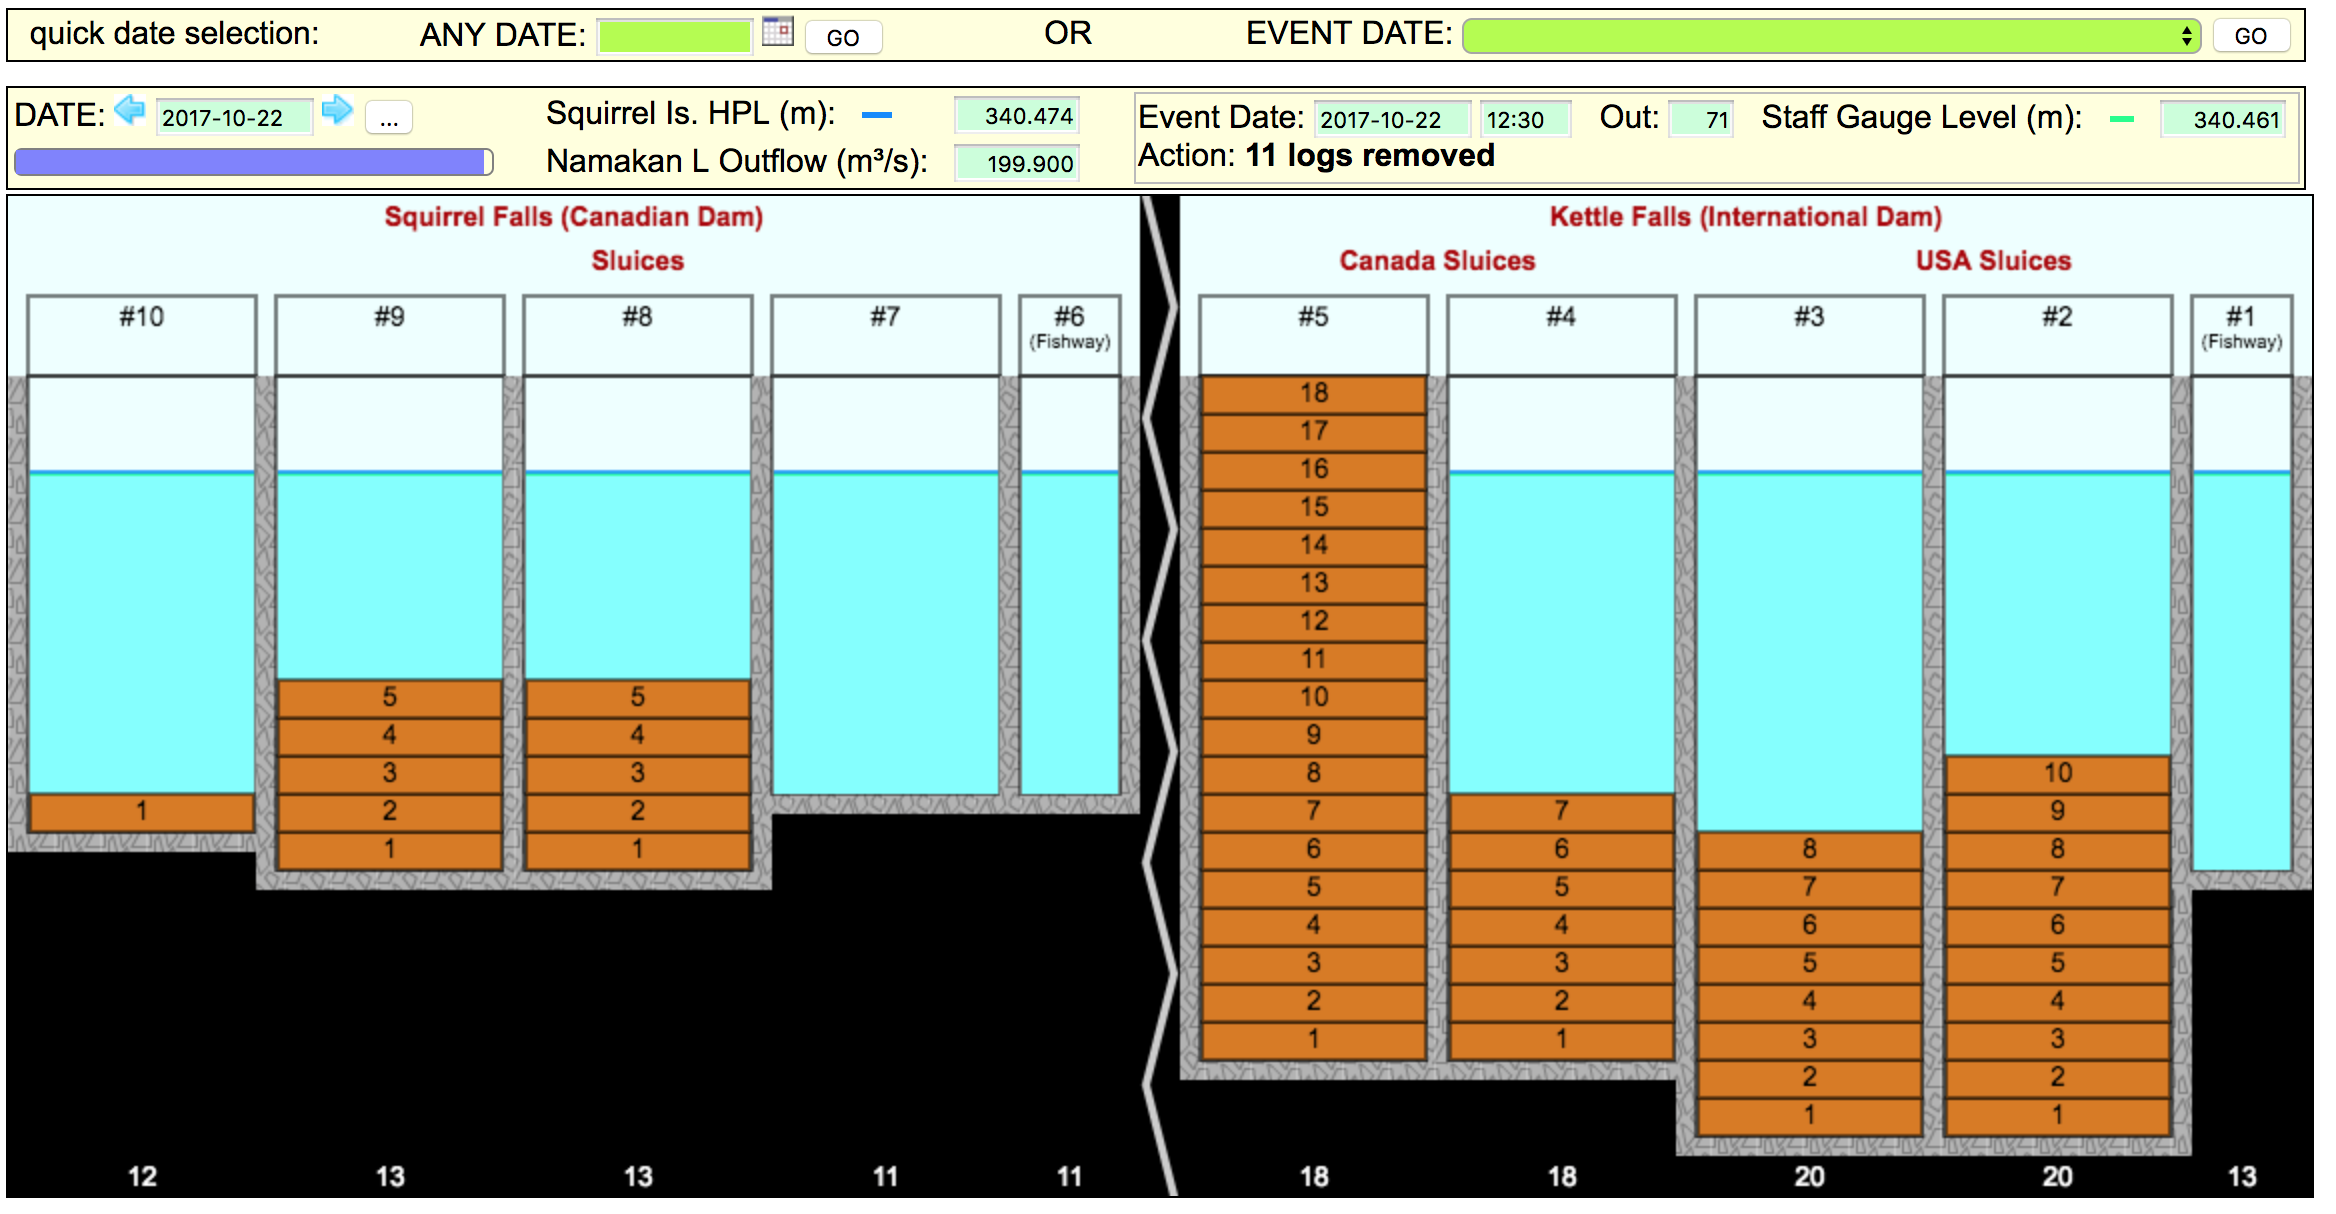
\includegraphics[width=0.9\paperwidth]{KettleFalls}
\end{center}

\end{frame}

%%%%%%%%%1%%%%%%%%%2%%%%%%%%%3%%%%%%%%%4%%%%%%%%%5%%%%%%%%%6
\begin{frame}{Rule Curves Establish Control Policy}

\begin{center}
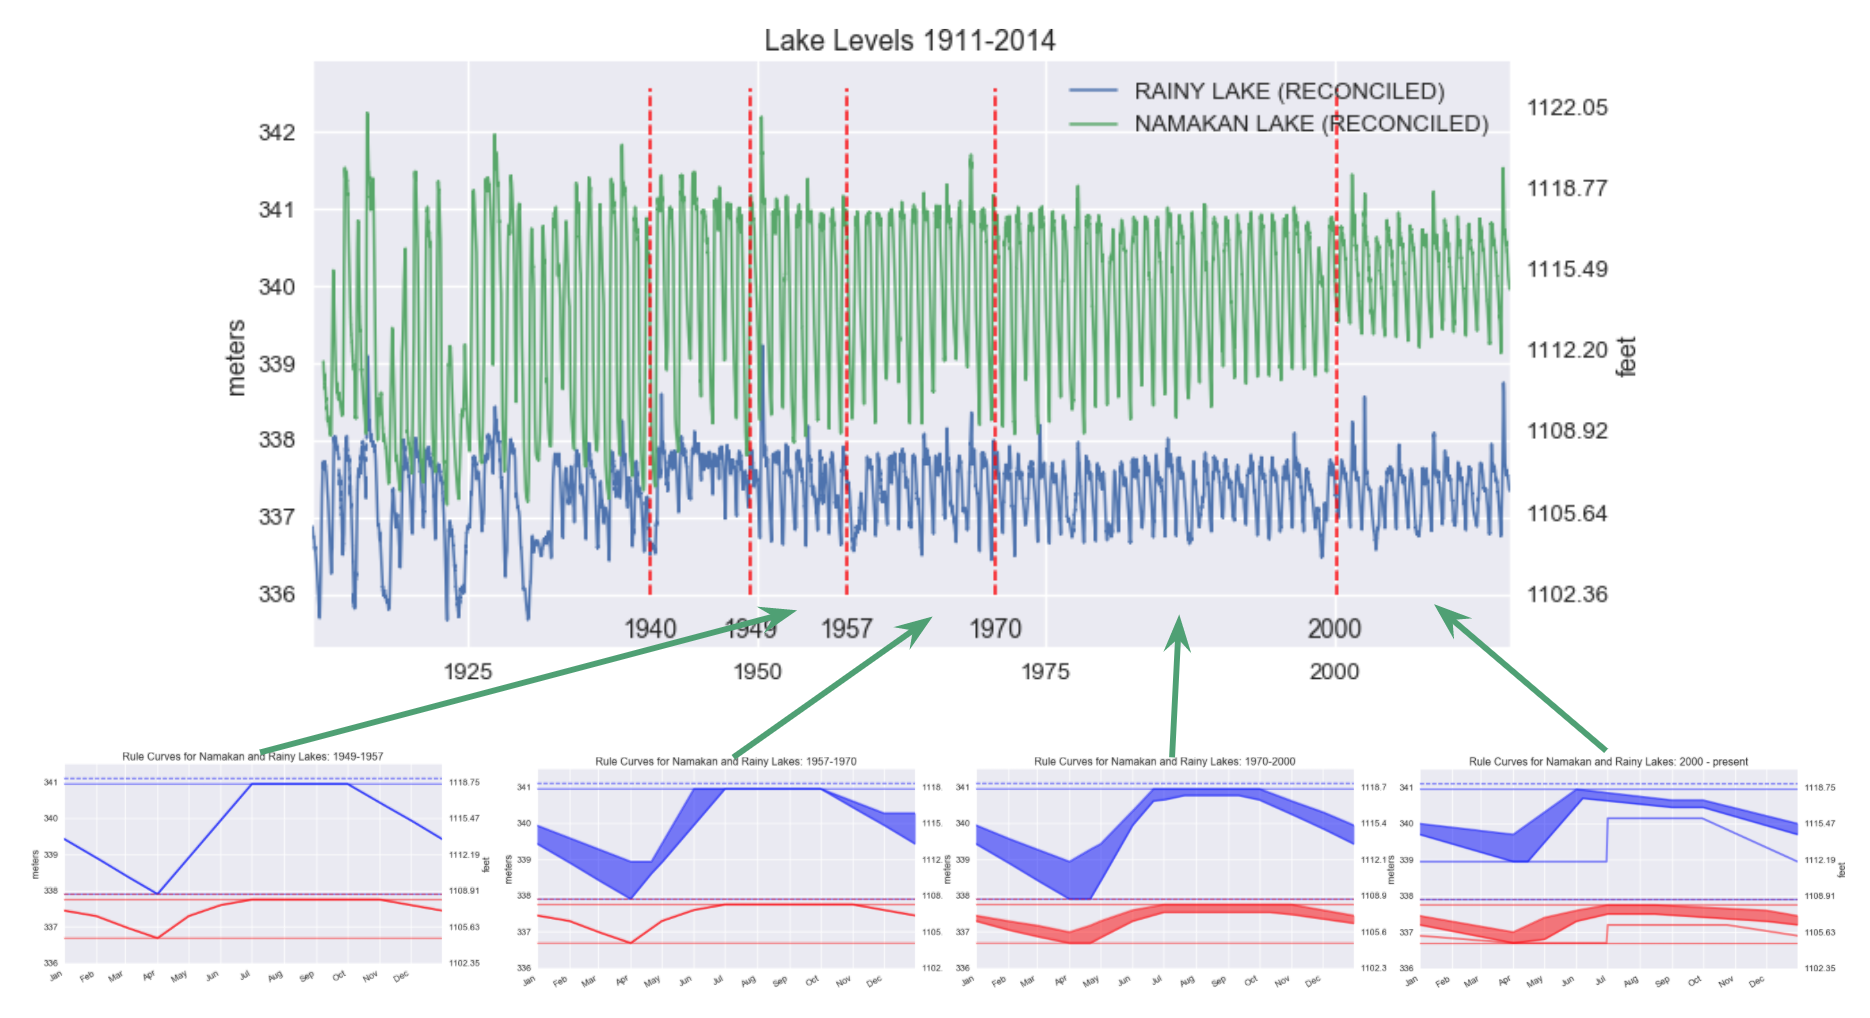
\includegraphics[width=0.9\paperwidth]{RuleCurves}
\end{center}
Rule Curves are established by the International Joint Commission by authority of the Boundary Waters Treaty of 1909.
\end{frame}

%%%%%%%%%1%%%%%%%%%2%%%%%%%%%3%%%%%%%%%4%%%%%%%%%5%%%%%%%%%6
% Section
%%%%%%%%%1%%%%%%%%%2%%%%%%%%%3%%%%%%%%%4%%%%%%%%%5%%%%%%%%%6
{\usebackgroundtemplate%
	{
\includegraphics[height=\paperheight]{background_grey.png}}
\section{Current Practice}
}

%%%%%%%%%1%%%%%%%%%2%%%%%%%%%3%%%%%%%%%4%%%%%%%%%5%%%%%%%%%6
\begin{frame}{Rule Curves}

\centering

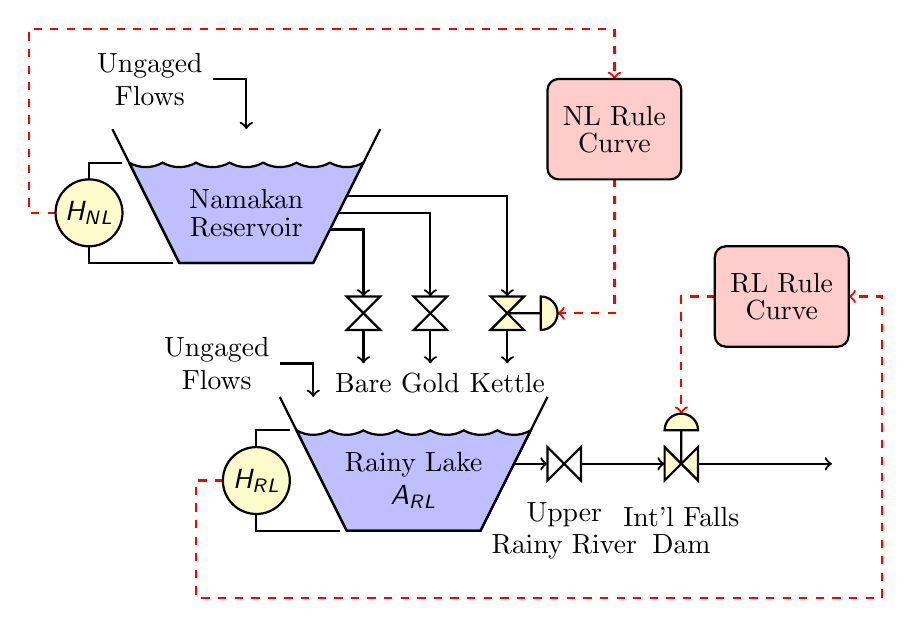
\begin{tikzpicture}[scale=0.85,thick]
\begin{sansmath}
  %\draw[step=1cm,gray,very thin] (0,0) grid (12,8);
  
  % Coordinates
  \coordinate (RL) at (3.5,2.5);
  \coordinate (NL) at (1,6.5); 
  \coordinate (Ranier) at (7.5,1.5);
  \coordinate (IFD) at (9.25,1.5);
  \coordinate (Kettle) at (6.9,4);
  \coordinate (Gold) at (5.75,4);
  \coordinate (Bare) at (4.75,4);
  \coordinate (control) at (11,4);
  \coordinate (control2) at (8.5,6.5);
  
  % Control lines
  \draw[dashed,->,color=red] (RL)++(-0.35,-1.25)--++(-0.9,0)--++(0,-1.75) 
    --++(10.25,0)--++(0,4.5)--++(-0.5,0);
  \draw[dashed,->,color=red] (control)--++(-1.5,0)--++(0,-1.75);
  \draw[dashed,->,color=red] (NL)++(-0.35,-1.25)--++(-0.9,0)--++(0,2.75)
    --++(8.75,0)--++(0,-0.75);
  \draw[dashed,->,color=red] (control2)--++(0,-2.75)--++(-0.85,0);
    
  % Valve Symbols 
  \draw[fill=yellow!20] (IFD)--++(0,0.25)--++(0.5,-0.5)--++(0,0.5)
    --++(-0.5,-0.5)--++(0,0.25)
    ++(0.25,0)--++(0,0.5)--++(0.25,0) arc(0:180:0.25) --++(0.25,0);
  \draw (IFD)++(0.25,-1) node {\shortstack{Int'l Falls \\ Dam}};
  
  \draw (Ranier)--++(0,0.25)--++(0.5,-0.5)--++(0,0.5)--++(-0.5,-0.5)--++(0,0.25);
  \draw (Ranier)++(0.25,-1) node {\shortstack{Upper\\ Rainy River}};
  
  \draw[fill=yellow!20] (Kettle)--++(0.25,0)--++(-0.5,-0.5)--++(0.5,0)--++(-0.5,0.5)--++(0.25,0)
    ++(0,-0.25)--++(0.5,0)--++(0,-0.25) arc(-90:90:0.25cm)--++(0,-0.25);
  
  \draw (Gold)--++(0.25,0)--++(-0.5,-0.5)--++(0.5,0)--++(-0.5,0.5)--++(0.25,0);
  \draw (Bare)--++(0.25,0)--++(-0.5,-0.5)--++(0.5,0)--++(-0.5,0.5)--++(0.25,0);
 
  % Level Transmitter
  \draw (RL) ++(0.15,-0.5)--++(-0.5,0)--++(0,-1.5) --++(1.25,0);
  \draw[fill=yellow!20] (RL) ++(-0.35,-0.75) arc(-270:90:0.5cm) 
    ++(0,-0.5) node {$H_{RL}$};
        
  \draw (NL) ++(0.15,-0.5)--++(-0.5,0)--++(0,-1.5) --++(1.25,0);
  \draw[fill=yellow!20] (NL) ++(-0.35,-0.75) arc(-270:90:0.5cm) 
    ++(0,-0.5) node {$H_{NL}$};
  
  % Connectors
  \draw[<-] (Kettle)++(0,-1.0) node[below] {Kettle} --++(0,0.5);
  \draw[<-] (Kettle)--++(0,1.5)--++(-3,0);
  
  \draw[<-] (Gold)++(0,-1) node[below] {Gold} --++(0,0.5);
  \draw[<-] (Gold)--++(0,1.25)--++(-3,0);
  
  \draw[<-] (Bare)++(0,-1) node[below] {Bare} --++(0,0.5);
  \draw[<-] (Bare)--++(0,1.0)--++(-3,0);
  
  \draw[<-] (RL)++(0.5,0)--++(0,0.5)--++(-0.5,0) 
    node[left] {\shortstack{Ungaged \\ Flows}};
  \draw[<-] (NL)++(2,0)--++(0,0.75)--++(-0.5,0)
    node[left] {\shortstack{Ungaged \\ Flows}};
    
  \draw[<-] (Ranier)--++(-2,0);
  \draw[<-] (IFD)--++(-1.25,0);
  \draw[->] (IFD)++(0.5,0)--++(2,0);
  
  % Rainy Lake
  \draw[fill=blue!25] (RL) ++(0.25,-0.5)--++(0.75,-1.5)--++(2,0)--++(0.75,1.5)
    arc(-60:-120:0.5cm) arc(-60:-120:0.5cm) arc(-60:-120:0.5cm) arc(-60:-120:0.5cm)
    arc(-60:-120:0.5cm) arc(-60:-120:0.5cm) arc(-60:-120:0.5cm);
  \draw (RL)--++(1,-2)--++(2,0)--++(1,2);
  \draw (RL) ++(2,-1.25) node {\shortstack{Rainy Lake \\ $A_{RL}$}};

  % Namakan Lake
  \draw[fill=blue!25] (NL) ++(0.25,-0.5)--++(0.75,-1.5)--++(2,0)--++(0.75,1.5)
    arc(-60:-120:0.5cm) arc(-60:-120:0.5cm) arc(-60:-120:0.5cm) arc(-60:-120:0.5cm)
    arc(-60:-120:0.5cm) arc(-60:-120:0.5cm) arc(-60:-120:0.5cm);
  \draw (NL)--++(1,-2)--++(2,0)--++(1,2);
  \draw (NL) ++(2,-1.25) node {\shortstack{Namakan \\ Reservoir}};
  
  % Controller
  \draw[rounded corners,fill=red!20] (control) 
    +(-1,-0.75) rectangle +(1,0.75);
  \draw (control) node {\shortstack{RL Rule\\ Curve}};
    
  \draw[rounded corners,fill=red!20] (control2) 
    +(-1,-0.75) rectangle +(1,0.75);
  \draw (control2) node {\shortstack{NL Rule\\ Curve}};
      
\end{sansmath}
\end{tikzpicture}

\end{frame}

%%%%%%%%%1%%%%%%%%%2%%%%%%%%%3%%%%%%%%%4%%%%%%%%%5%%%%%%%%%6
\begin{frame}{Rule Curve Performance 1970--1999}

\begin{center}
\includegraphicscopyright[width=0.8\paperwidth]{RuleCurvePerformance1970-1999.png}{Source: \href{http://jckantor.github.io/Rainy-Lake-Hydrology/}{Github Repository for this paper.}}
\end{center}

\end{frame}

%%%%%%%%%1%%%%%%%%%2%%%%%%%%%3%%%%%%%%%4%%%%%%%%%5%%%%%%%%%6
\begin{frame}{Rule Curve Performance 2000--2014}

\begin{center}
\includegraphicscopyright[width=0.8\paperwidth]{RuleCurvePerformance2000-2010.png}{Source: \href{http://jckantor.github.io/Rainy-Lake-Hydrology/}{Github Repository for this paper.}}
\end{center}

\end{frame}

%%%%%%%%%1%%%%%%%%%2%%%%%%%%%3%%%%%%%%%4%%%%%%%%%5%%%%%%%%%6
\begin{frame}{Rule Curve Performance - Rainy Lake Levels}

\begin{center}
\includegraphicscopyright[width=0.75\paperwidth]{RLFreqStage.png}{Source: \href{http://jckantor.github.io/Rainy-Lake-Hydrology/}{Github Repository for this paper.}}
\end{center}

\end{frame}

%%%%%%%%%1%%%%%%%%%2%%%%%%%%%3%%%%%%%%%4%%%%%%%%%5%%%%%%%%%6
\begin{frame}{Increasing Frequency of Flooding Events}

\begin{center}
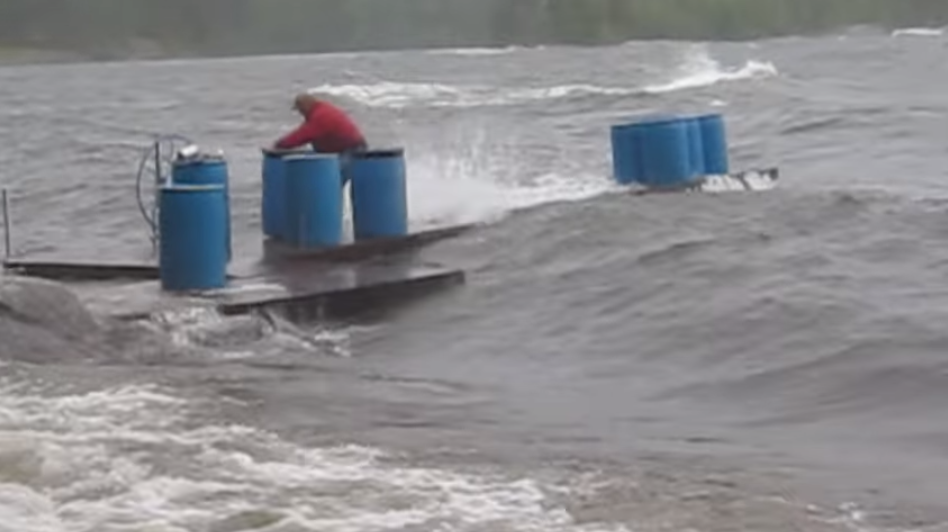
\includegraphics[width=0.75\paperwidth]{WaterBarrelsDock}
\end{center}

\end{frame}

%%%%%%%%%1%%%%%%%%%2%%%%%%%%%3%%%%%%%%%4%%%%%%%%%5%%%%%%%%%6
% Section 
%%%%%%%%%1%%%%%%%%%2%%%%%%%%%3%%%%%%%%%4%%%%%%%%%5%%%%%%%%%6

{\usebackgroundtemplate%
	{
\includegraphics[height=\paperheight]{background_grey.png}}
\section{Predictive Control 1. Implementing Rule Curves}
}

%%%%%%%%%1%%%%%%%%%2%%%%%%%%%3%%%%%%%%%4%%%%%%%%%5%%%%%%%%%6
\begin{frame}{Model Predictive Control for Rainy Lake}

\centering

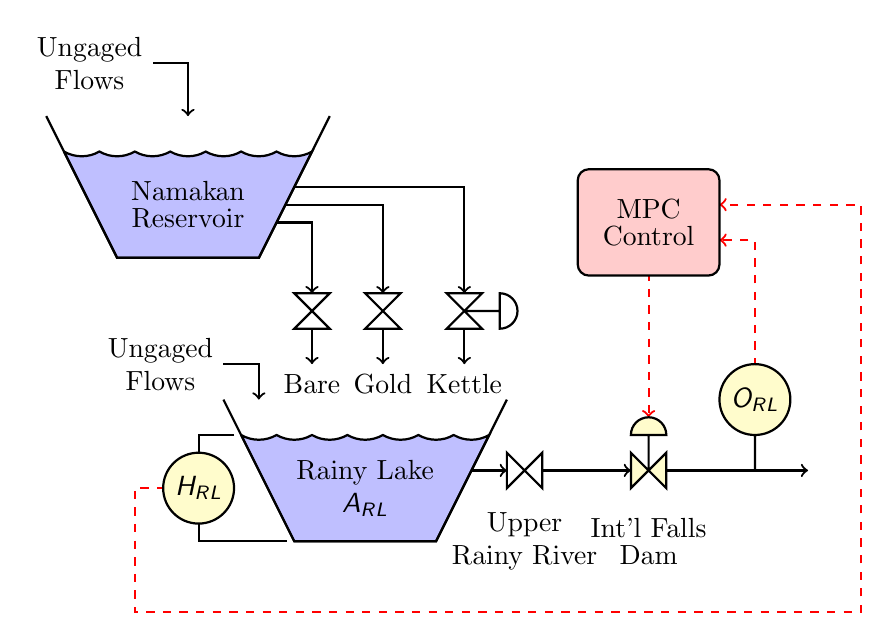
\begin{tikzpicture}[scale=0.9,thick]
\begin{sansmath}
  %\draw[step=1cm,gray,very thin] (0,0) grid (12,8);
  
  % Coordinates
  \coordinate (RL) at (3.5,2.5);
  \coordinate (NL) at (1,6.5); 
  \coordinate (Ranier) at (7.5,1.5);
  \coordinate (IFD) at (9.25,1.5);
  \coordinate (FT) at (11,1.5);
  \coordinate (Kettle) at (6.9,4);
  \coordinate (Gold) at (5.75,4);
  \coordinate (Bare) at (4.75,4);
  \coordinate (control) at (9.5,5);
  
  % Control lines
  \draw[dashed,->,color=red] (RL)++(-0.35,-1.25)--++(-0.9,0)--++(0,-1.75) 
    --++(10.25,0)--++(0,5.75)--++(-2,0);
  \draw[dashed,->,color=red] (FT)++(0,1)--++(0,2.25)--++(-0.5,0);
  \draw[dashed,->,color=red] (control)--++(0,-2.75);
  
  % Valve Symbols 
  \draw[fill=yellow!20] (IFD)--++(0,0.25)--++(0.5,-0.5)--++(0,0.5)
    --++(-0.5,-0.5)--++(0,0.25)
    ++(0.25,0)--++(0,0.5)--++(0.25,0) arc(0:180:0.25) --++(0.25,0);
  \draw (IFD)++(0.25,-1) node {\shortstack{Int'l Falls \\ Dam}};
  
  \draw (Ranier)--++(0,0.25)--++(0.5,-0.5)--++(0,0.5)--++(-0.5,-0.5)--++(0,0.25);
  \draw (Ranier)++(0.25,-1) node {\shortstack{Upper\\ Rainy River}};
  
  \draw (Kettle)--++(0.25,0)--++(-0.5,-0.5)--++(0.5,0)--++(-0.5,0.5)--++(0.25,0)
    ++(0,-0.25)--++(0.5,0)--++(0,-0.25) arc(-90:90:0.25cm)--++(0,-0.25);
  
  \draw (Gold)--++(0.25,0)--++(-0.5,-0.5)--++(0.5,0)--++(-0.5,0.5)--++(0.25,0);
  \draw (Bare)--++(0.25,0)--++(-0.5,-0.5)--++(0.5,0)--++(-0.5,0.5)--++(0.25,0);
  
  % Flow Transmitter
  \draw[fill=yellow!20] (FT)--++(0,0.5) arc(-90:270:0.5cm) ++(0,0.5) node {$O_{RL}$};
 
  % Level Transmitter
  \draw (RL) ++(0.15,-0.5)--++(-0.5,0)--++(0,-1.5) --++(1.25,0);
  \draw[fill=yellow!20] (RL) ++(-0.35,-0.75) arc(-270:90:0.5cm) 
    ++(0,-0.5) node {$H_{RL}$};
  
  % Connectors
  \draw[<-] (Kettle)++(0,-1.0) node[below] {Kettle} --++(0,0.5);
  \draw[<-] (Kettle)--++(0,1.5)--++(-3,0);
  
  \draw[<-] (Gold)++(0,-1) node[below] {Gold} --++(0,0.5);
  \draw[<-] (Gold)--++(0,1.25)--++(-3,0);
  
  \draw[<-] (Bare)++(0,-1) node[below] {Bare} --++(0,0.5);
  \draw[<-] (Bare)--++(0,1.0)--++(-3,0);
  
  \draw[<-] (RL)++(0.5,0)--++(0,0.5)--++(-0.5,0) 
    node[left] {\shortstack{Ungaged \\ Flows}};
  \draw[<-] (NL)++(2,0)--++(0,0.75)--++(-0.5,0)
    node[left] {\shortstack{Ungaged \\ Flows}};
    
  \draw[<-] (Ranier)--++(-2,0);
  \draw[<-] (IFD)--++(-1.25,0);
  \draw[->] (IFD)++(0.5,0)--++(2,0);
  
  % Rainy Lake
  \draw[fill=blue!25] (RL) ++(0.25,-0.5)--++(0.75,-1.5)--++(2,0)--++(0.75,1.5)
    arc(-60:-120:0.5cm) arc(-60:-120:0.5cm) arc(-60:-120:0.5cm) arc(-60:-120:0.5cm)
    arc(-60:-120:0.5cm) arc(-60:-120:0.5cm) arc(-60:-120:0.5cm);
  \draw (RL)--++(1,-2)--++(2,0)--++(1,2);
  \draw (RL) ++(2,-1.25) node {\shortstack{Rainy Lake \\ $A_{RL}$}};

  % Namakan Lake
  \draw[fill=blue!25] (NL) ++(0.25,-0.5)--++(0.75,-1.5)--++(2,0)--++(0.75,1.5)
    arc(-60:-120:0.5cm) arc(-60:-120:0.5cm) arc(-60:-120:0.5cm) arc(-60:-120:0.5cm)
    arc(-60:-120:0.5cm) arc(-60:-120:0.5cm) arc(-60:-120:0.5cm);
  \draw (NL)--++(1,-2)--++(2,0)--++(1,2);
  \draw (NL) ++(2,-1.25) node {\shortstack{Namakan \\ Reservoir}};
  
  % Controller
    \draw[rounded corners,fill=red!20] (control) 
      +(-1,-0.75) rectangle +(1,0.75);
    \draw (control) node {\shortstack{MPC\\ Control}};
      
\end{sansmath}
\end{tikzpicture}

\end{frame}

%%%%%%%%%1%%%%%%%%%2%%%%%%%%%3%%%%%%%%%4%%%%%%%%%5%%%%%%%%%6
\begin{frame}{Upper Rainy River Discharge Characteristics}

\begin{center}
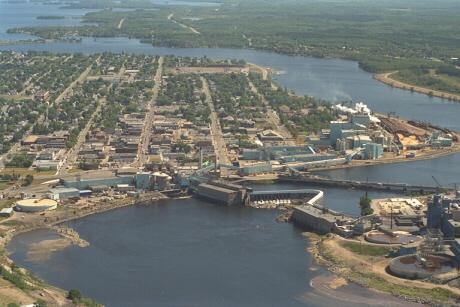
\includegraphics[width=0.75\paperwidth]{mill.jpg}
\end{center}

\end{frame} 

%%%%%%%%%1%%%%%%%%%2%%%%%%%%%3%%%%%%%%%4%%%%%%%%%5%%%%%%%%%6
\begin{frame}{Upper Rainy River Discharge Characteristics}

\begin{center}
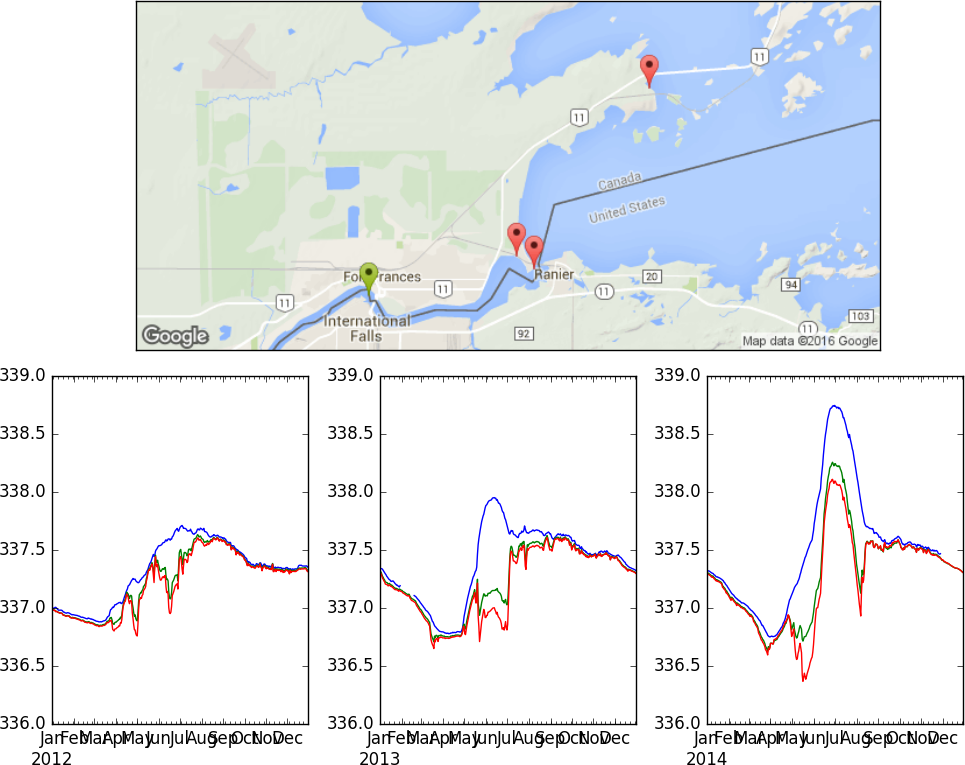
\includegraphics[width=0.75\paperwidth]{RainyRiverConstrictions.png}
\end{center}

\end{frame} 

%%%%%%%%%1%%%%%%%%%2%%%%%%%%%3%%%%%%%%%4%%%%%%%%%5%%%%%%%%%6
\begin{frame}{Upper Rainy River Discharge Characteristics}

\begin{center}
\includegraphicscopyright[width=0.75\paperwidth]{RainyRiverDischarge_Fit.png}{Source: \href{http://jckantor.github.io/Rainy-Lake-Hydrology/}{Github Repository for this paper.}}
\end{center}

\end{frame} 

%%%%%%%%%1%%%%%%%%%2%%%%%%%%%3%%%%%%%%%4%%%%%%%%%5%%%%%%%%%6
\begin{frame}{Maximum Controllable Inflows}

\begin{center}
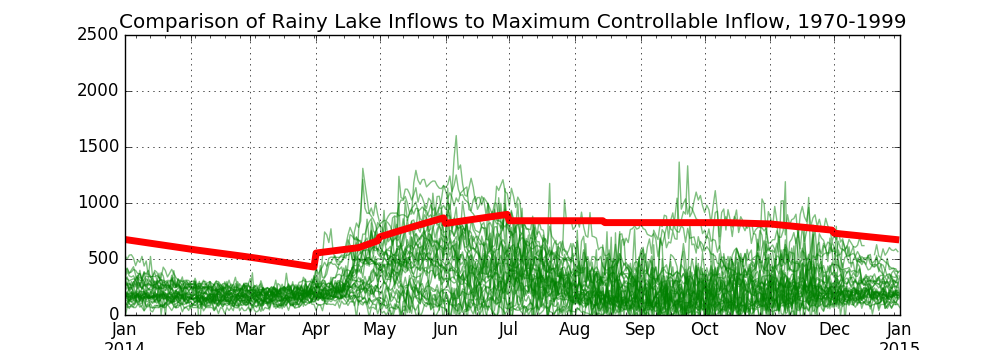
\includegraphics[width=0.8\paperwidth]{RLMaxFlow1970.png}

\includegraphicscopyright[width=0.8\paperwidth]{RLMaxFlow2000.png}{Source: \href{http://jckantor.github.io/Rainy-Lake-Hydrology/}{Github Repository for this paper.}}

\end{center}

\end{frame}

%%%%%%%%%1%%%%%%%%%2%%%%%%%%%3%%%%%%%%%4%%%%%%%%%5%%%%%%%%%6
\begin{frame}{Uncontrollable Inflow Frequency}

\begin{center}
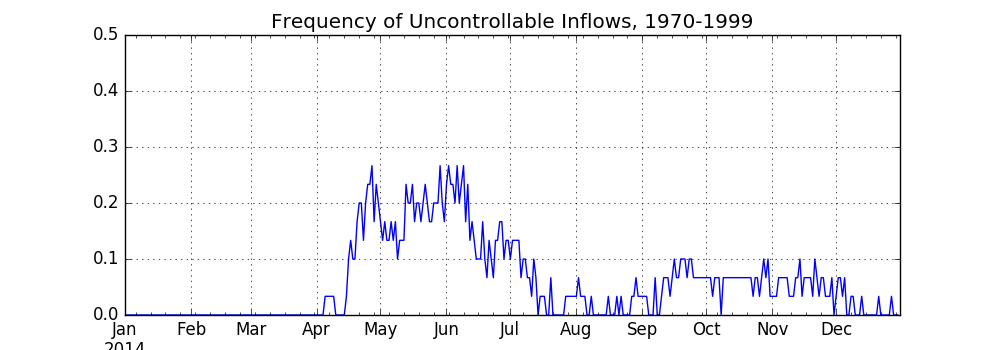
\includegraphics[width=0.8\paperwidth]{RLMaxFlowFreq1970.png}

\includegraphicscopyright[width=0.8\paperwidth]{RLMaxFlowFreq2000.png}{Source: \href{http://jckantor.github.io/Rainy-Lake-Hydrology/}{Github Repository for this paper.}}
\end{center}

\end{frame}

%%%%%%%%%1%%%%%%%%%2%%%%%%%%%3%%%%%%%%%4%%%%%%%%%5%%%%%%%%%6
\begin{frame}{Inflow Estimation}

\begin{center}
\includegraphicscopyright[width=0.8\paperwidth]{RainyLakeInflows.png}{Source: \href{http://jckantor.github.io/Rainy-Lake-Hydrology/}{Github Repository for this paper.}}
\end{center}

\end{frame}

%%%%%%%%%1%%%%%%%%%2%%%%%%%%%3%%%%%%%%%4%%%%%%%%%5%%%%%%%%%6
\begin{frame}{Matlab/Simulink Implementation}

\begin{center}
\includegraphicscopyright[width=0.85\paperwidth]{RLSim_Model.png}{Source: \href{http://jckantor.github.io/Rainy-Lake-Hydrology/}{Github Repository for this paper.}}
\end{center}

\end{frame}

%%%%%%%%%1%%%%%%%%%2%%%%%%%%%3%%%%%%%%%4%%%%%%%%%5%%%%%%%%%6
\begin{frame}{Simulation Results}

\vfill
\centering
\includegraphicscopyright[width=0.8\paperwidth]{RLSim_Results.png}{Source: \href{http://jckantor.github.io/Rainy-Lake-Hydrology/}{Github Repository for this paper.}}
\vfill

\end{frame}

%%%%%%%%%1%%%%%%%%%2%%%%%%%%%3%%%%%%%%%4%%%%%%%%%5%%%%%%%%%6
\begin{frame}{Simulation Results}

\vfill
\centering
\includegraphicscopyright[width=0.75\paperwidth]{RuleCurvePerformance1970-1999_sim.png}{Source: \href{http://jckantor.github.io/Rainy-Lake-Hydrology/}{Github Repository for this paper.}}\vfill

\end{frame}

%%%%%%%%%1%%%%%%%%%2%%%%%%%%%3%%%%%%%%%4%%%%%%%%%5%%%%%%%%%6
\begin{frame}{Simulation Results}

\vfill
\centering
\includegraphicscopyright[width=0.75\paperwidth]{RuleCurvePerformance2000-2014_sim.png}{Source: \href{http://jckantor.github.io/Rainy-Lake-Hydrology/}{Github Repository for this paper.}}
\vfill

\end{frame}

%%%%%%%%%1%%%%%%%%%2%%%%%%%%%3%%%%%%%%%4%%%%%%%%%5%%%%%%%%%6
\begin{frame}{Simulation Results - Rainy Lake Levels}

\vfill
\centering
\includegraphicscopyright[width=0.75\paperwidth]{RLFreqStage_sim.png}{Source: \href{http://jckantor.github.io/Rainy-Lake-Hydrology/}{Github Repository for this paper.}}
\vfill

\end{frame}

%%%%%%%%%1%%%%%%%%%2%%%%%%%%%3%%%%%%%%%4%%%%%%%%%5%%%%%%%%%6
\begin{frame}{Summer 2015}

In 2015, Dam Operators committed to more careful control using feedback principles augmented with inflow and level forecasting information.

One outcome was a record crop of wild rice
\begin{columns}
	\begin{column}{0.5\textwidth}
		\begin{center}
			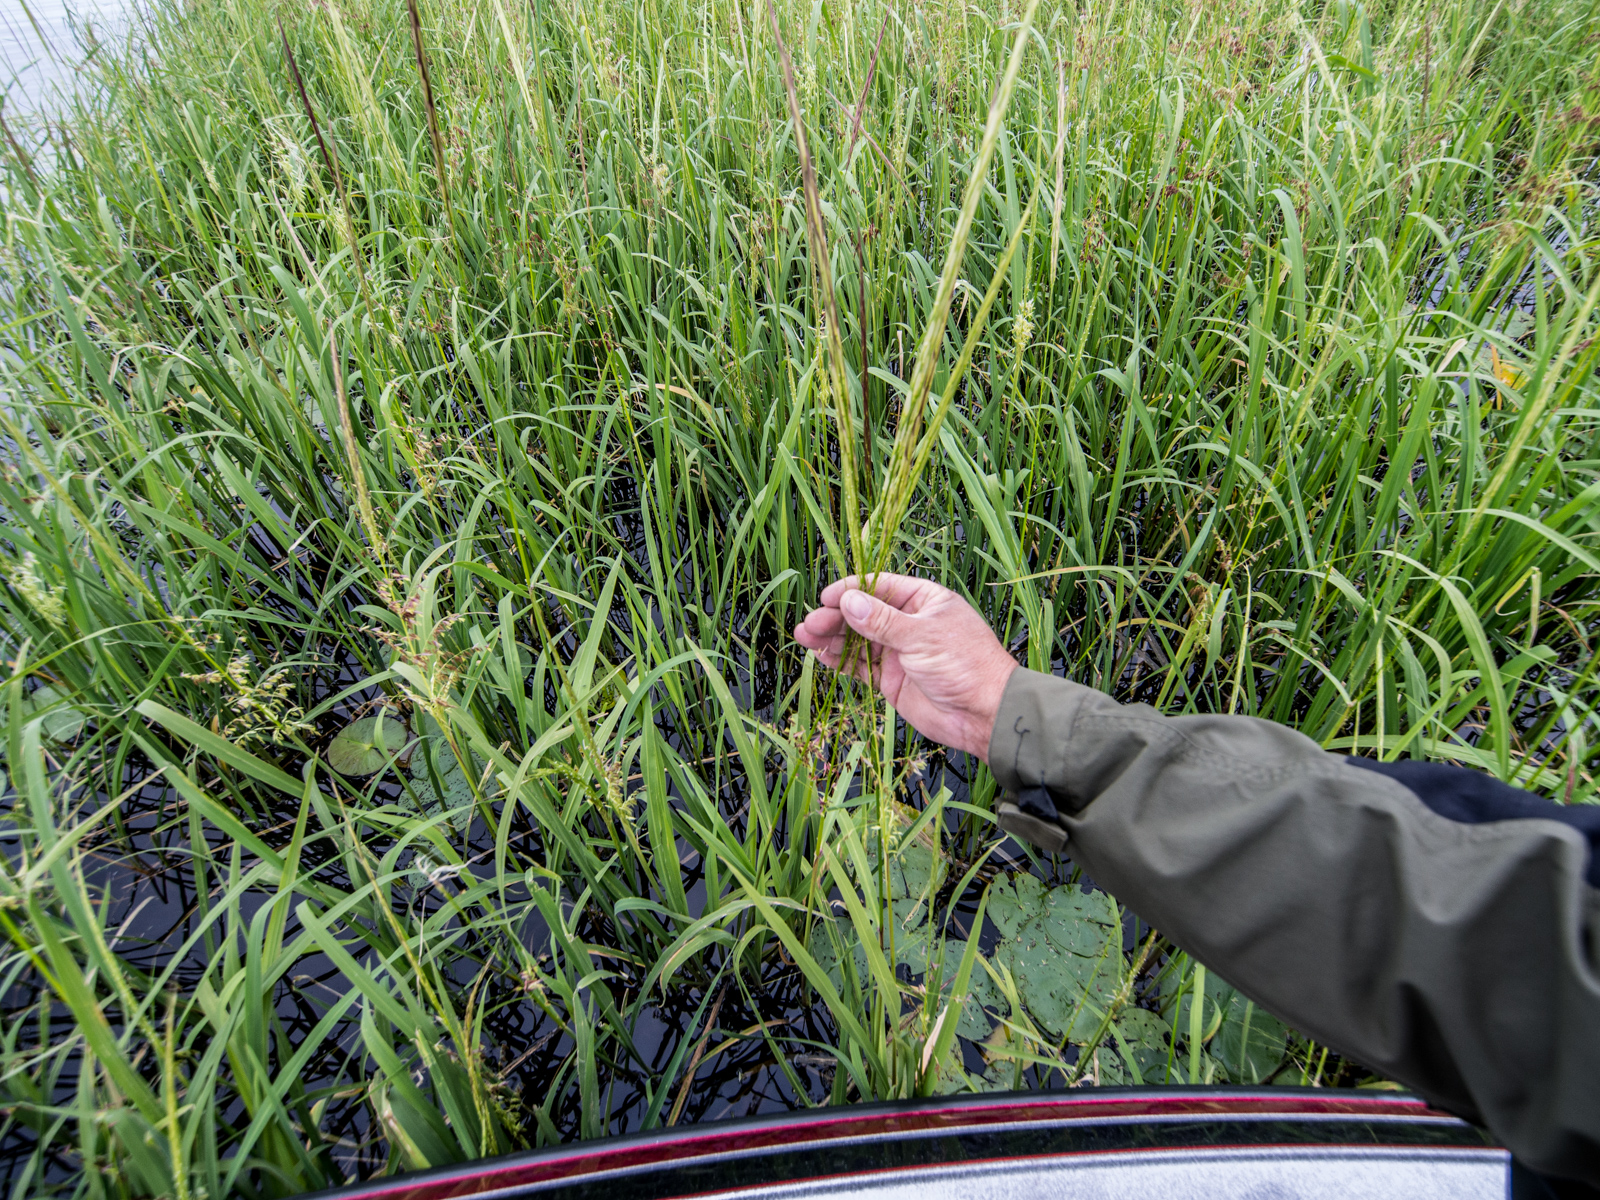
\includegraphics[width=\textwidth]{20150804_194209.jpg}
		\end{center}
	\end{column}
	\begin{column}{0.5\textwidth}
		\begin{center}
			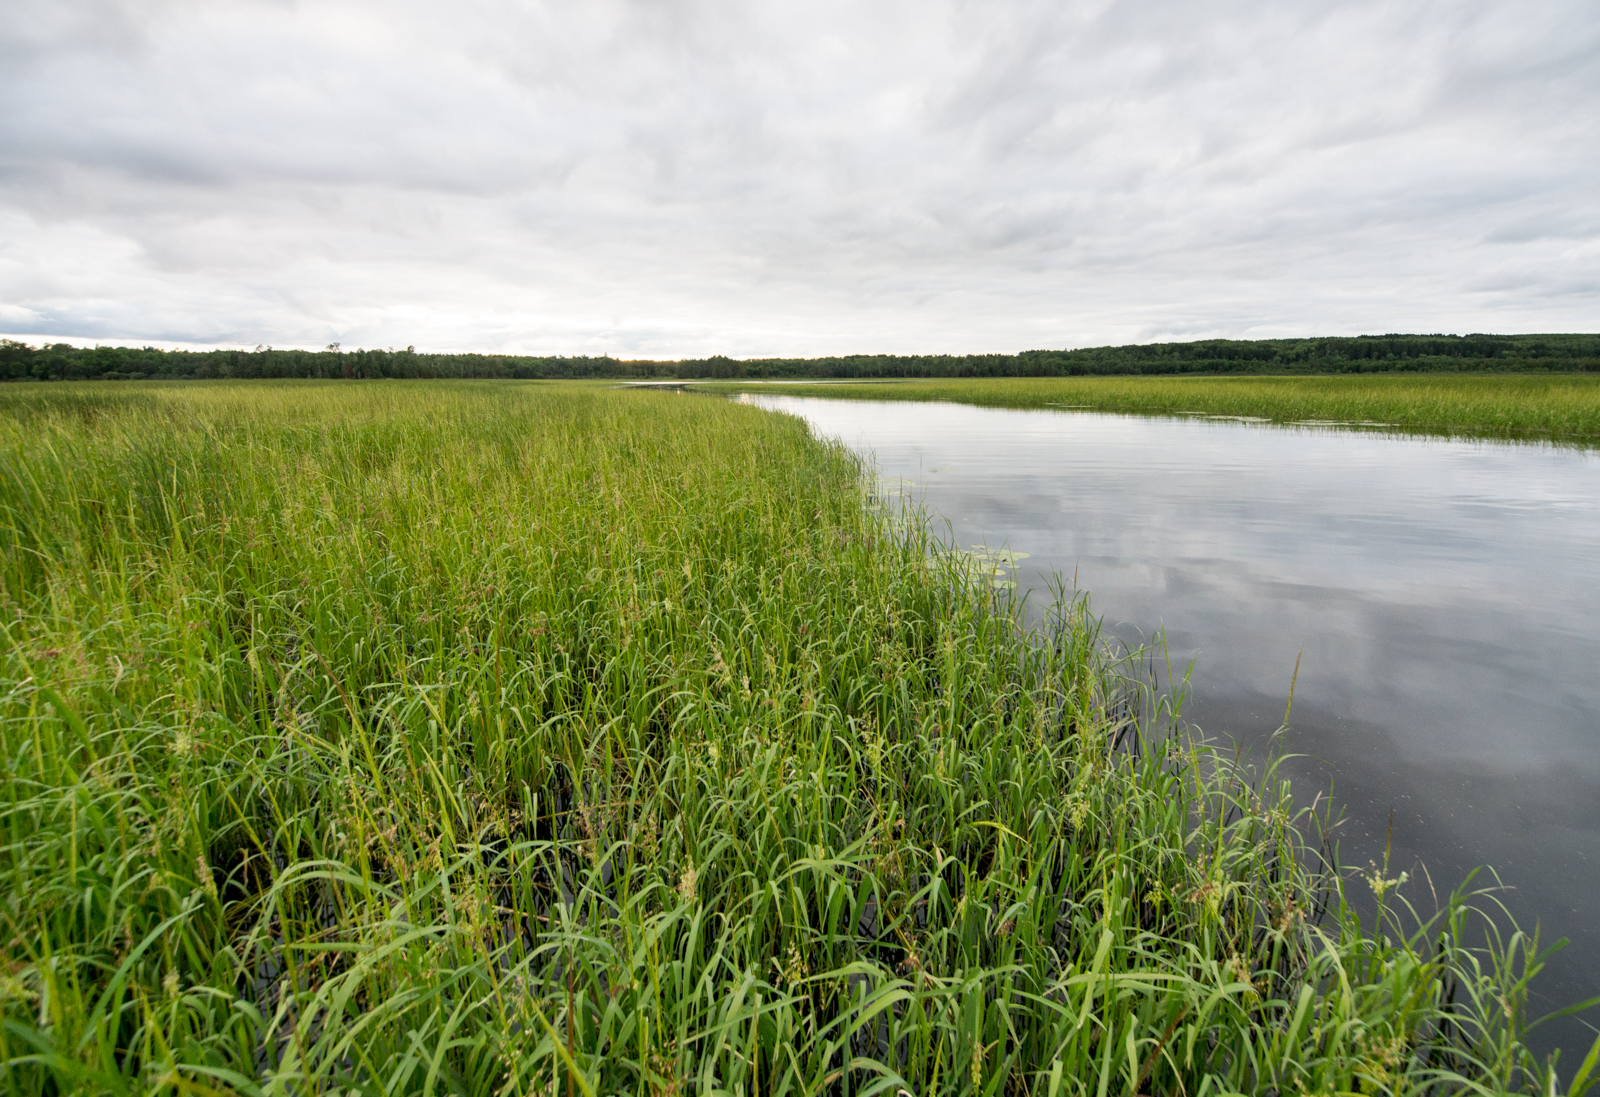
\includegraphics[width=\textwidth]{20150804_194303.jpg}
		\end{center}
	\end{column}
\end{columns}
Other outcomes were increased downstream bank erosion.
\end{frame}

%%%%%%%%%1%%%%%%%%%2%%%%%%%%%3%%%%%%%%%4%%%%%%%%%5%%%%%%%%%6
% Section
%%%%%%%%%1%%%%%%%%%2%%%%%%%%%3%%%%%%%%%4%%%%%%%%%5%%%%%%%%%6

{\usebackgroundtemplate%
	{
\includegraphics[width=\paperwidth]{background_grey.png}}
\section{Predictive Contol 2. Adaptive Rule Curves}
}

%%%%%%%%%1%%%%%%%%%2%%%%%%%%%3%%%%%%%%%4%%%%%%%%%5%%%%%%%%%6
\begin{frame}{Freshet and Ice Out}

\begin{center}
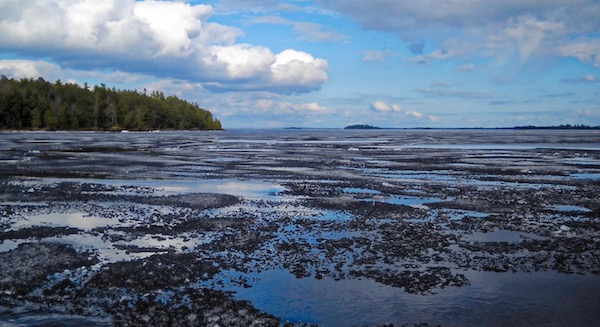
\includegraphics[width=0.8\paperwidth]{DSCN0059_.jpg}
\end{center}

The Spring Freshet followed by Ice Out is the start of the annual fill cycle.

\end{frame}

%%%%%%%%%1%%%%%%%%%2%%%%%%%%%3%%%%%%%%%4%%%%%%%%%5%%%%%%%%%6
\begin{frame}{Significance of Variable Ice Out}

\begin{center}
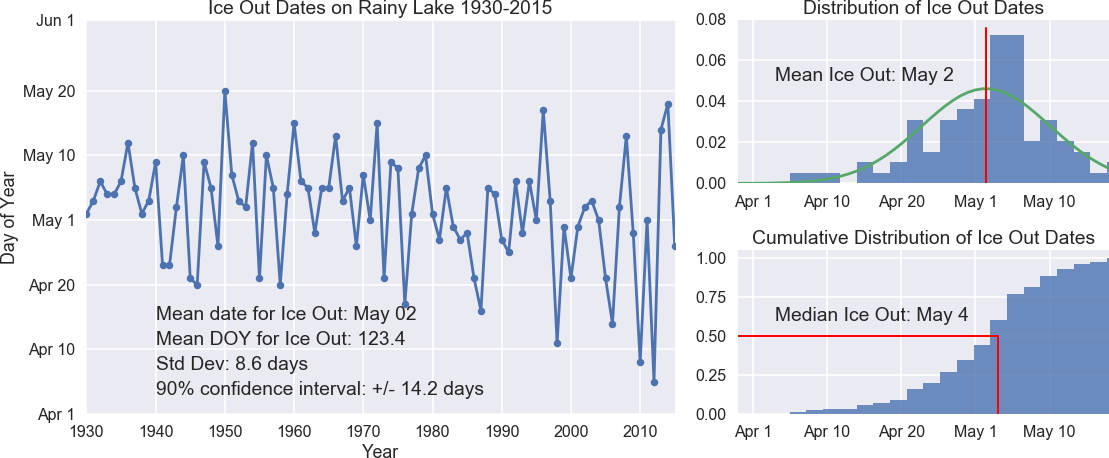
\includegraphics[width=0.8\paperwidth]{IceOutData.png}
\end{center}

Ice out is correlated with the Spring inflows of water.

\end{frame}

%%%%%%%%%1%%%%%%%%%2%%%%%%%%%3%%%%%%%%%4%%%%%%%%%5%%%%%%%%%6
\begin{frame}{Significance of Variable Ice Out}

\begin{center}
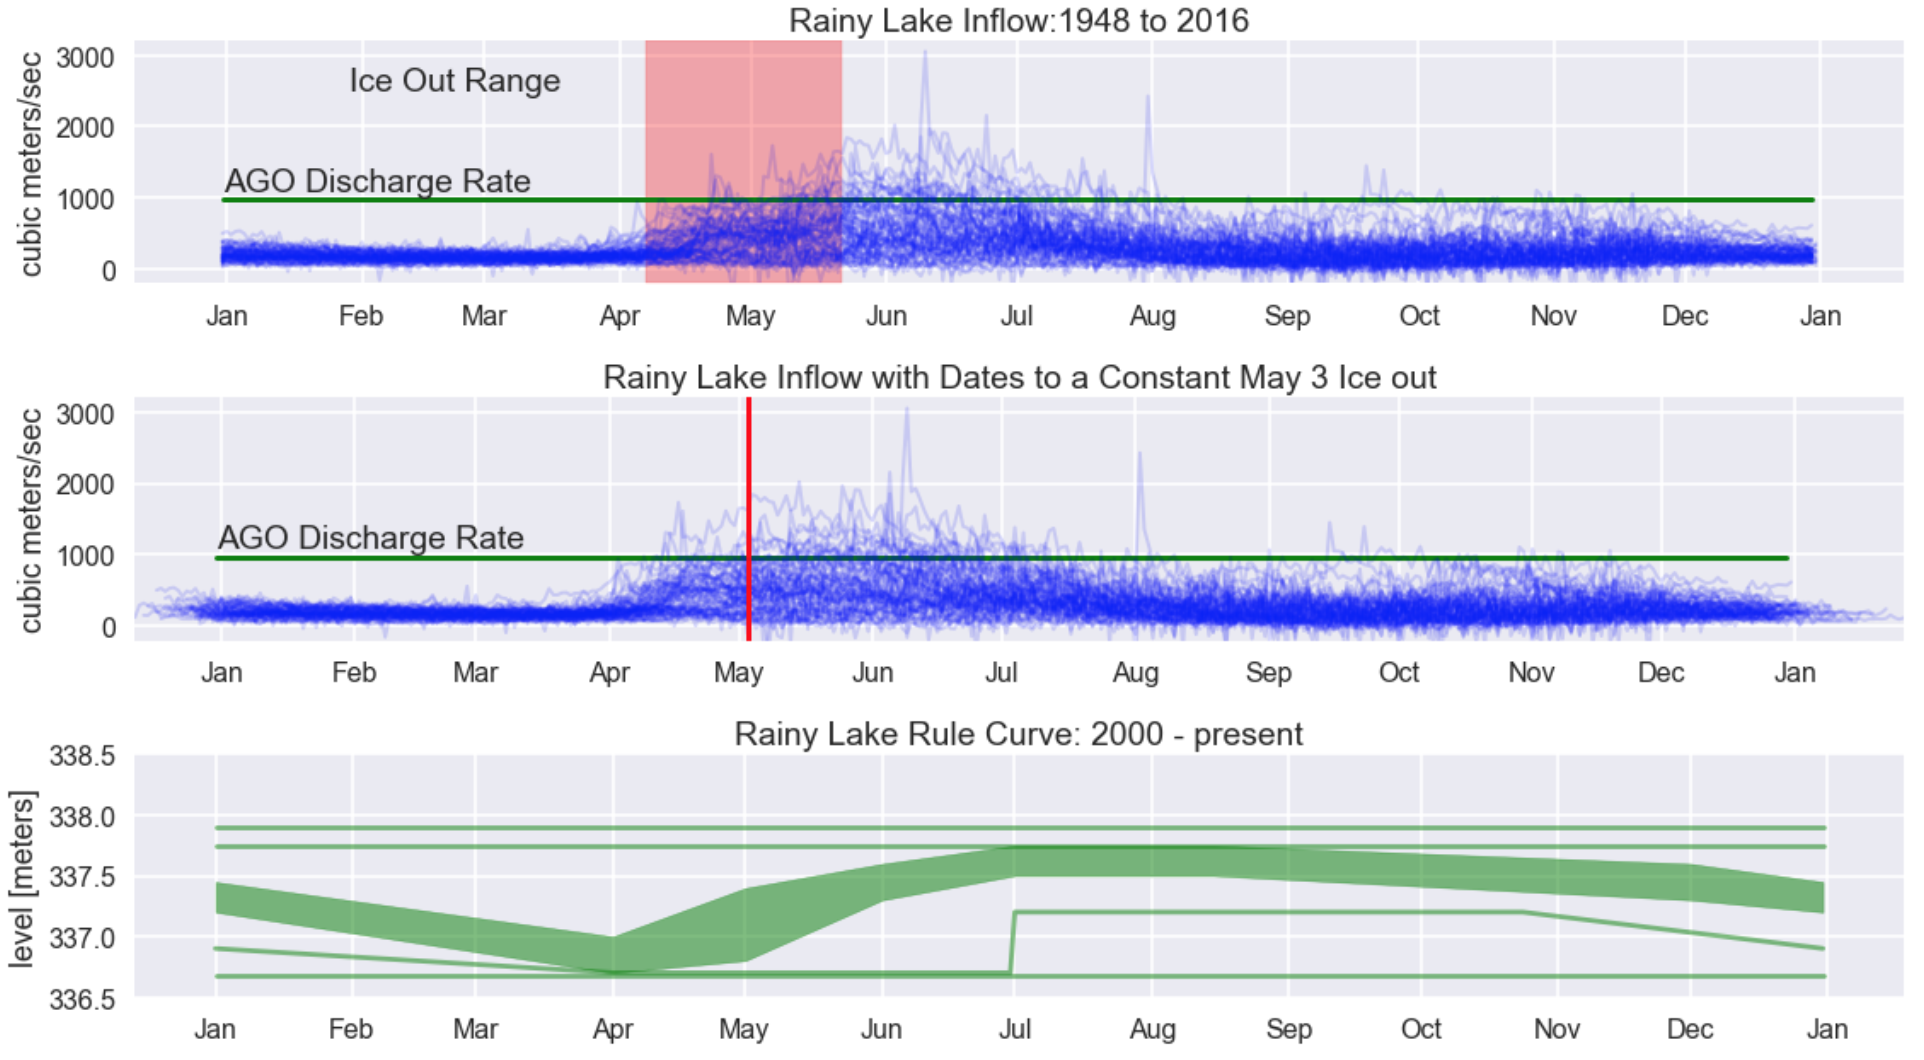
\includegraphics[width=0.8\paperwidth]{IceOutInflow2.png}
\end{center}

\end{frame}

%%%%%%%%%1%%%%%%%%%2%%%%%%%%%3%%%%%%%%%4%%%%%%%%%5%%%%%%%%%6
\begin{frame}{Trendlines}

\begin{center}
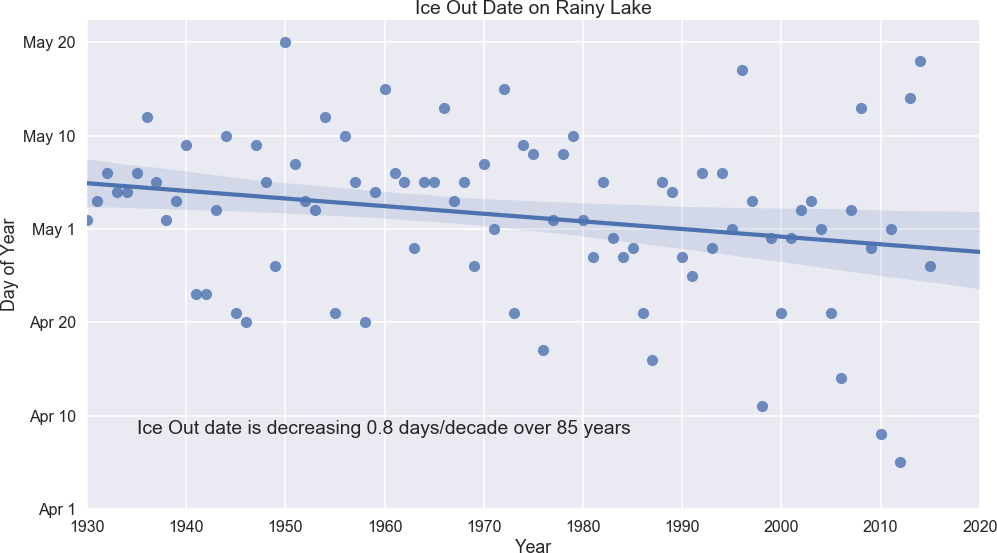
\includegraphics[width=0.8\paperwidth]{IceOutTrendLine.png}
\end{center}

\end{frame}

%%%%%%%%%1%%%%%%%%%2%%%%%%%%%3%%%%%%%%%4%%%%%%%%%5%%%%%%%%%6
\begin{frame}{Consistent with Global Warming}

\begin{center}
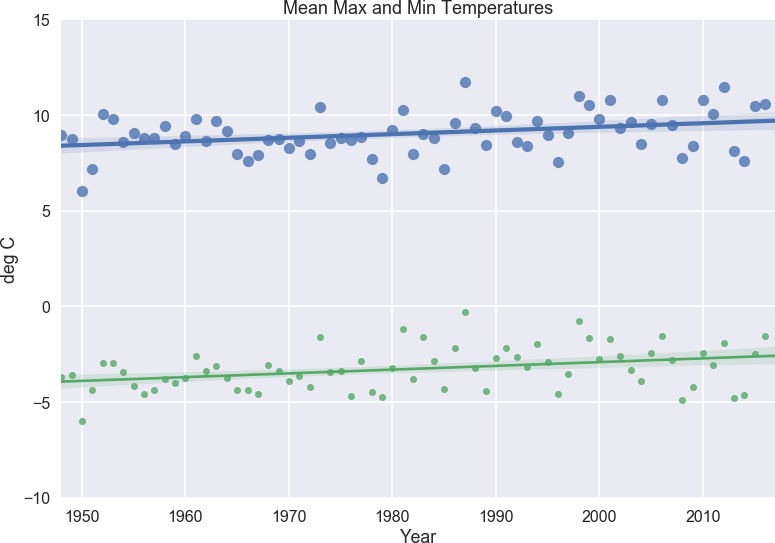
\includegraphics[width=0.8\paperwidth]{TempTrend.png}
\end{center}

\end{frame}

%%%%%%%%%1%%%%%%%%%2%%%%%%%%%3%%%%%%%%%4%%%%%%%%%5%%%%%%%%%6
\begin{frame}{Wind Distribution is Changing}

\begin{center}
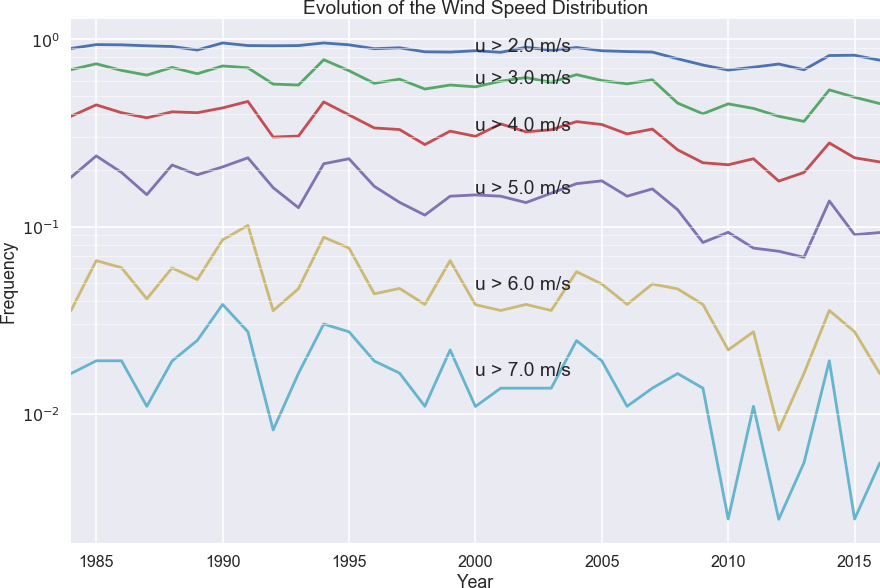
\includegraphics[width=0.8\paperwidth]{WindDistribution.png}
\end{center}

\end{frame}

%%%%%%%%%1%%%%%%%%%2%%%%%%%%%3%%%%%%%%%4%%%%%%%%%5%%%%%%%%%6
\begin{frame}{Consistent with Global Stilling}

\begin{center}
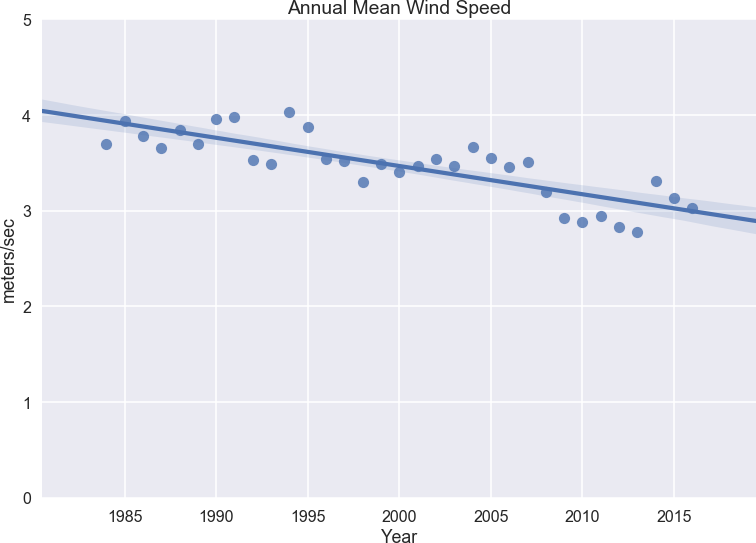
\includegraphics[width=0.8\paperwidth]{WindTrendLine.png}
\end{center}

\end{frame}

%%%%%%%%%1%%%%%%%%%2%%%%%%%%%3%%%%%%%%%4%%%%%%%%%5%%%%%%%%%6
\begin{frame}{Consistent with Global Stilling}

\begin{center}
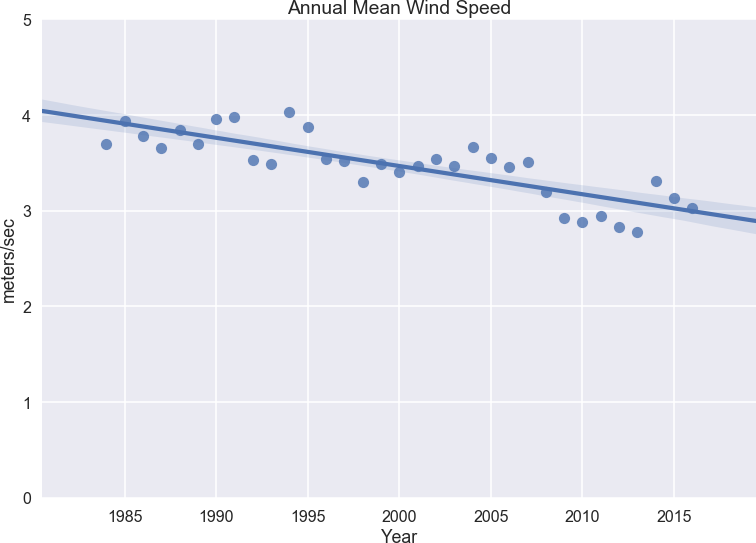
\includegraphics[width=0.8\paperwidth]{WindTrendLine.png}
\end{center}

\end{frame}

%%%%%%%%%1%%%%%%%%%2%%%%%%%%%3%%%%%%%%%4%%%%%%%%%5%%%%%%%%%6
\begin{frame}{March 1 Predictor}

\begin{center}
\includegraphicscopyright[width=0.85\paperwidth]{IceOut_PredictionMarch.png}{Source: \href{http://jckantor.github.io/Rainy-Lake-Hydrology/}{Github Repository for this paper.}}
\end{center}

Predictor fitted using Elastic Net Regression with ENSO, PDO,
local weather station temperature data for preceding 3 months.

Formal recommendation to the International Joint Commission for Adaptive Management of the Rainy Lake Basin.

\end{frame}


%%%%%%%%%1%%%%%%%%%2%%%%%%%%%3%%%%%%%%%4%%%%%%%%%5%%%%%%%%%6
% Section
%%%%%%%%%1%%%%%%%%%2%%%%%%%%%3%%%%%%%%%4%%%%%%%%%5%%%%%%%%%6

{\usebackgroundtemplate%
	{
\includegraphics[width=\paperwidth]{background_grey.png}}
\section{Predictive Contol 3. Ecosystem}
}

%%%%%%%%%1%%%%%%%%%2%%%%%%%%%3%%%%%%%%%4%%%%%%%%%5%%%%%%%%%6
\begin{frame}{Key Ecological Considerations}

\begin{center}
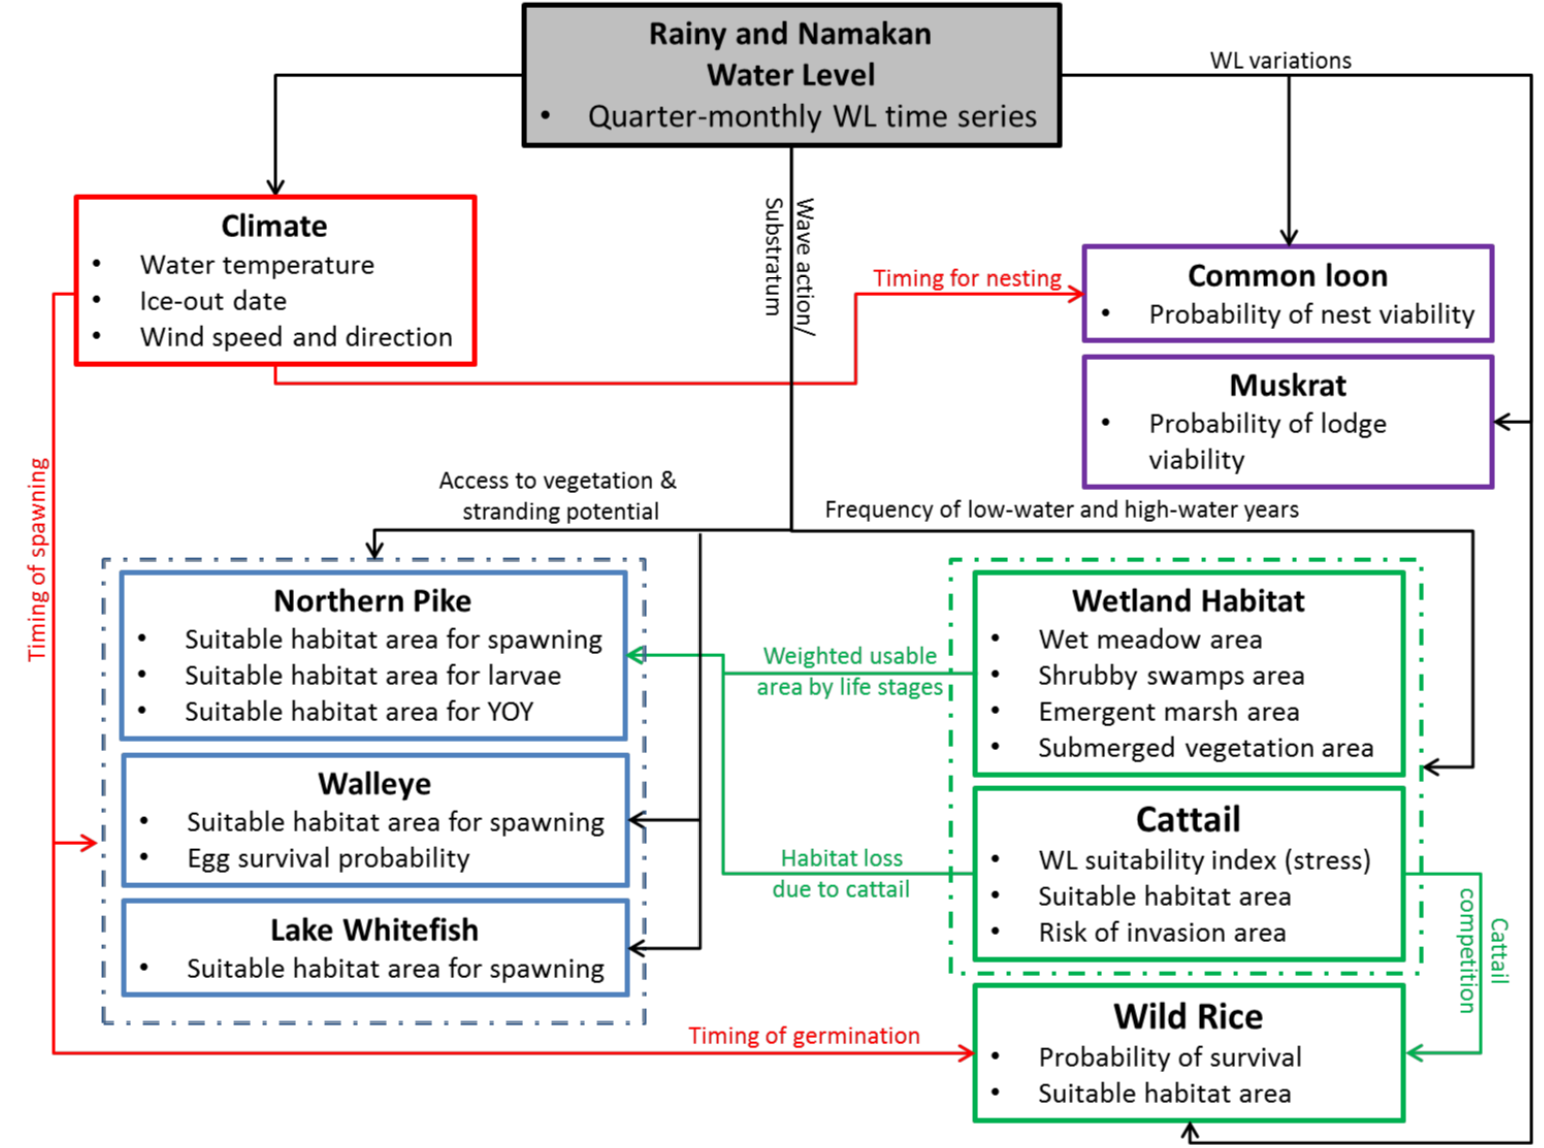
\includegraphics[width=0.8\paperwidth]{MorinEcology.png}
\end{center}

\end{frame}

%%%%%%%%%1%%%%%%%%%2%%%%%%%%%3%%%%%%%%%4%%%%%%%%%5%%%%%%%%%6
\begin{frame}{Submerged Vegetation}

\begin{center}
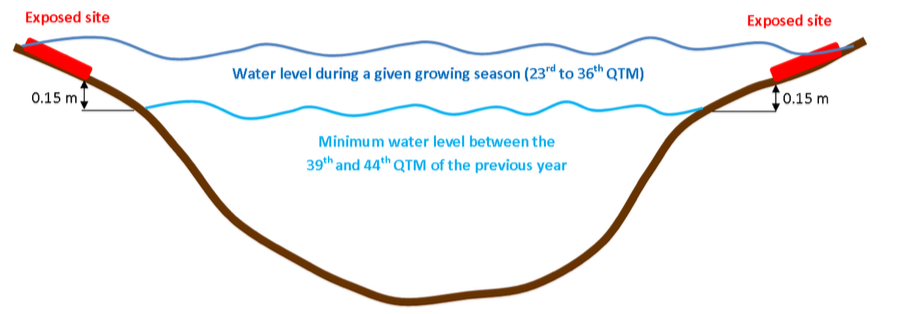
\includegraphics[width=0.8\paperwidth]{MorinVeg.png}
\end{center}

\end{frame}

%%%%%%%%%1%%%%%%%%%2%%%%%%%%%3%%%%%%%%%4%%%%%%%%%5%%%%%%%%%6
\begin{frame}{Loons}

\begin{center}
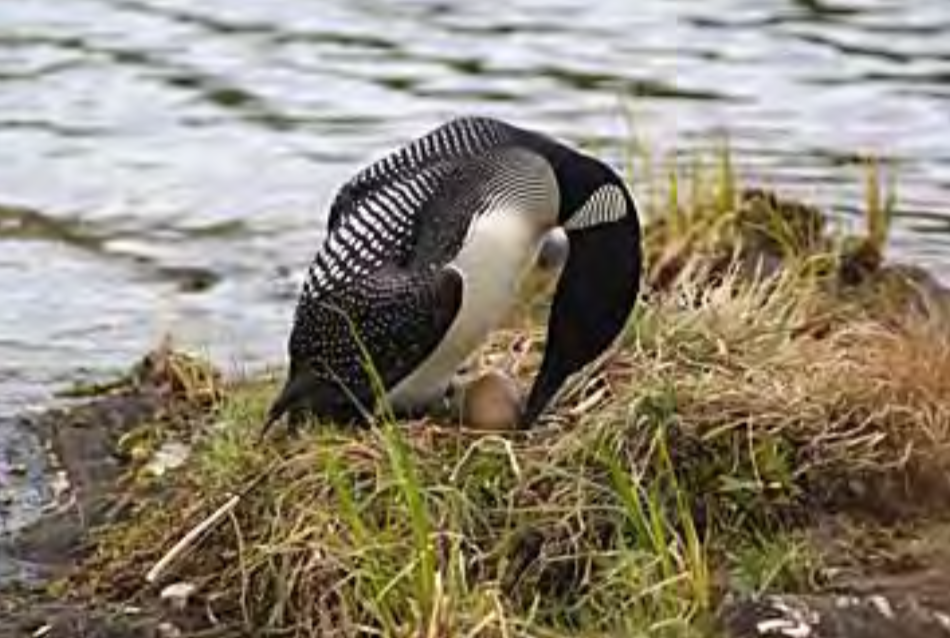
\includegraphics[width=0.8\paperwidth]{MorinLoon.png}
\end{center}

\end{frame}

%%%%%%%%%1%%%%%%%%%2%%%%%%%%%3%%%%%%%%%4%%%%%%%%%5%%%%%%%%%6
\begin{frame}{Muskrat}

\begin{center}
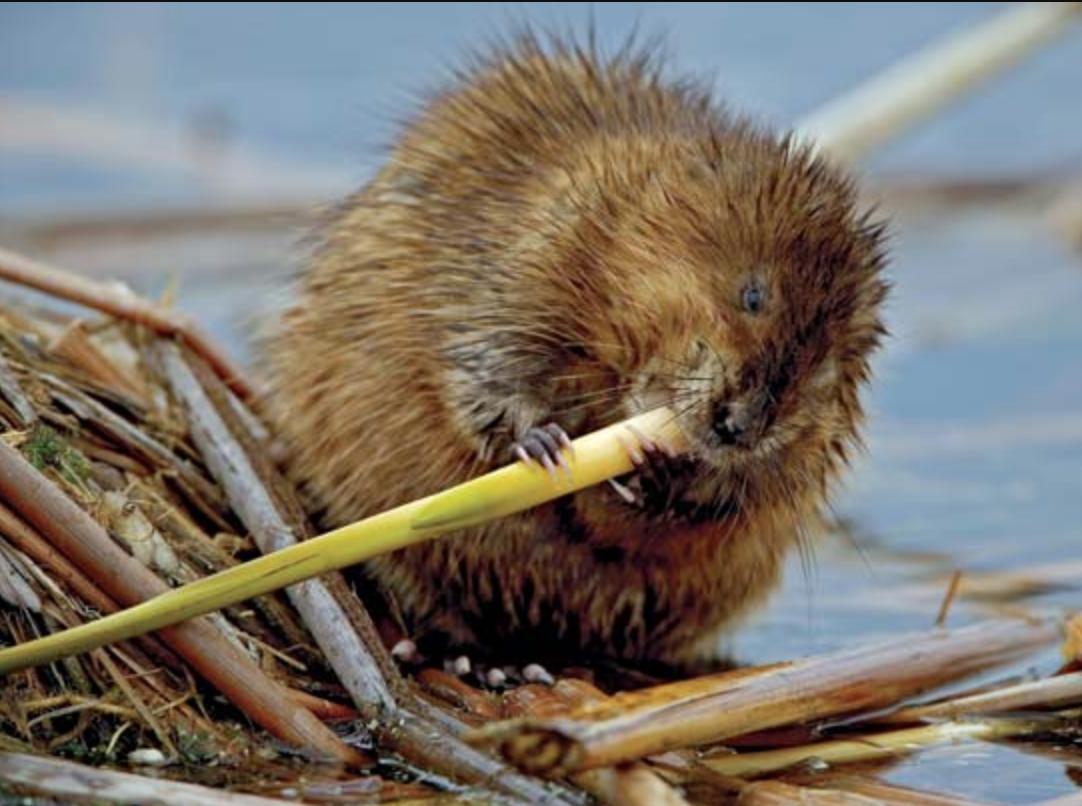
\includegraphics[width=0.8\paperwidth]{Muskrat.png}
\end{center}

\end{frame}

%%%%%%%%%1%%%%%%%%%2%%%%%%%%%3%%%%%%%%%4%%%%%%%%%5%%%%%%%%%6
\begin{frame}{Muskrat}

\begin{center}
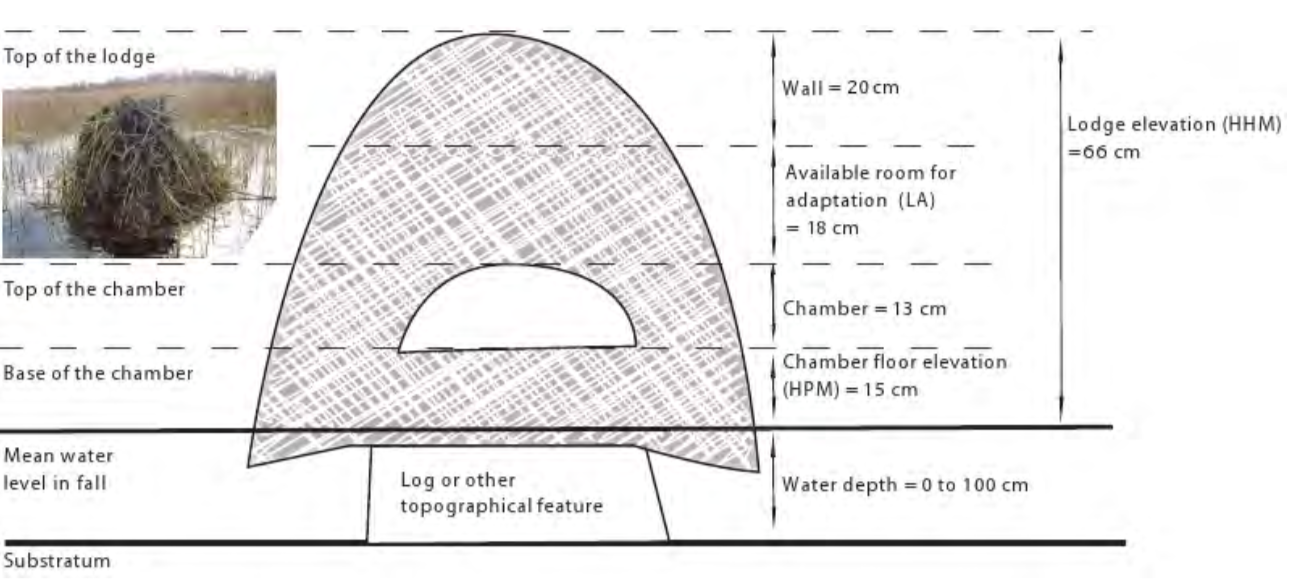
\includegraphics[width=0.8\paperwidth]{MorinMuskrat.png}
\end{center}

\end{frame}

%%%%%%%%%1%%%%%%%%%2%%%%%%%%%3%%%%%%%%%4%%%%%%%%%5%%%%%%%%%6
\begin{frame}{Wild Rice}

\begin{center}
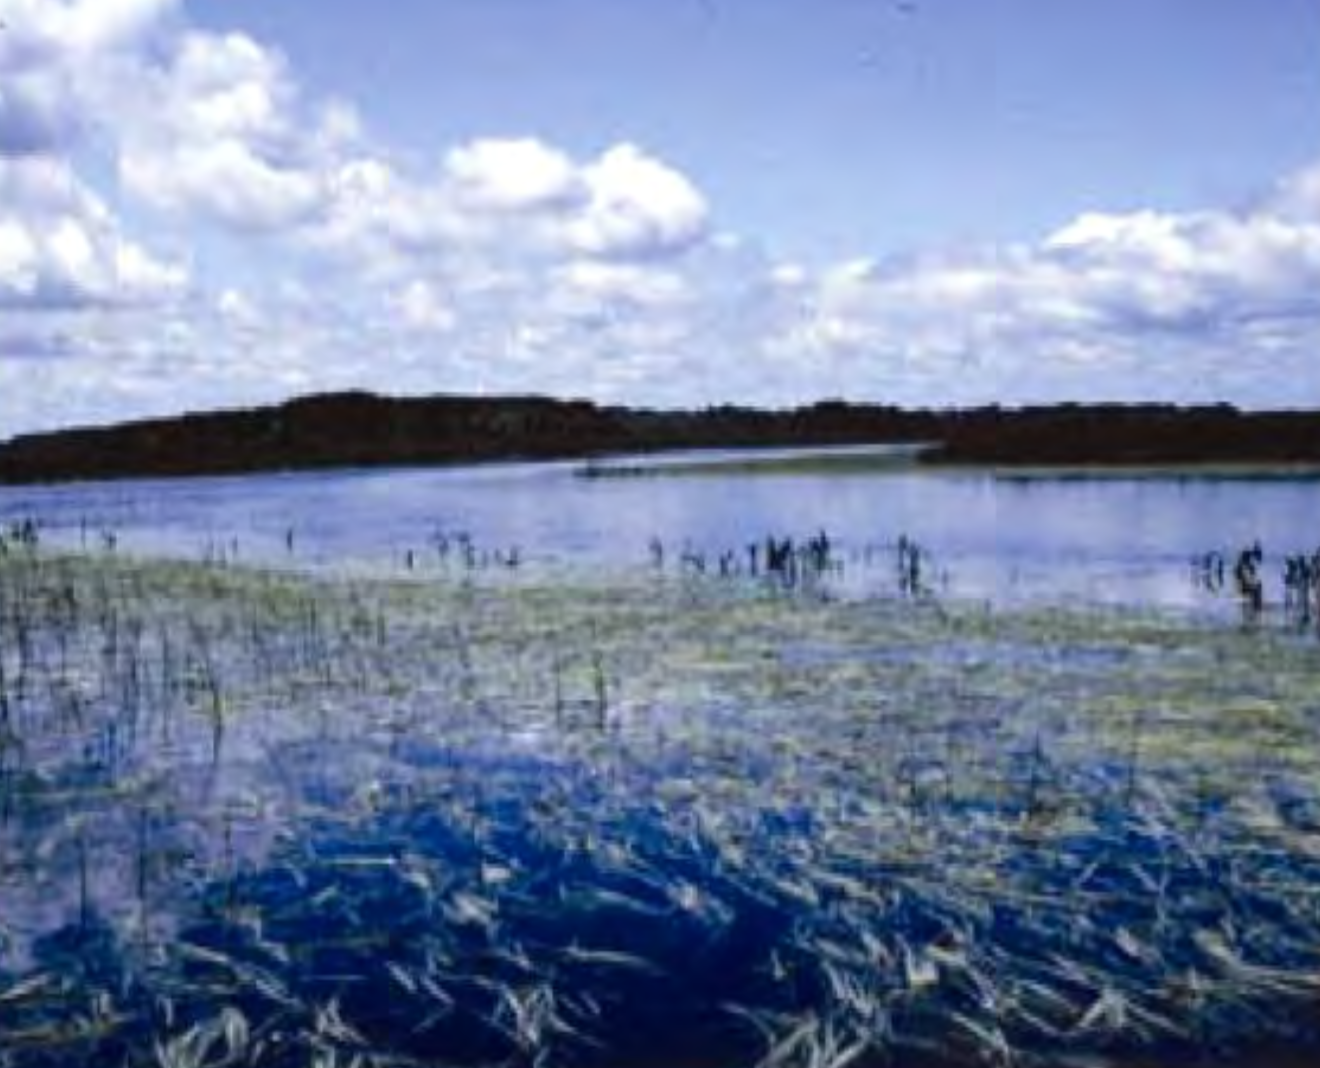
\includegraphics[width=0.8\paperwidth]{MorinWR.png}
\end{center}

\end{frame}

%%%%%%%%%1%%%%%%%%%2%%%%%%%%%3%%%%%%%%%4%%%%%%%%%5%%%%%%%%%6
\begin{frame}{Predictive Control Considerations}

\begin{center}
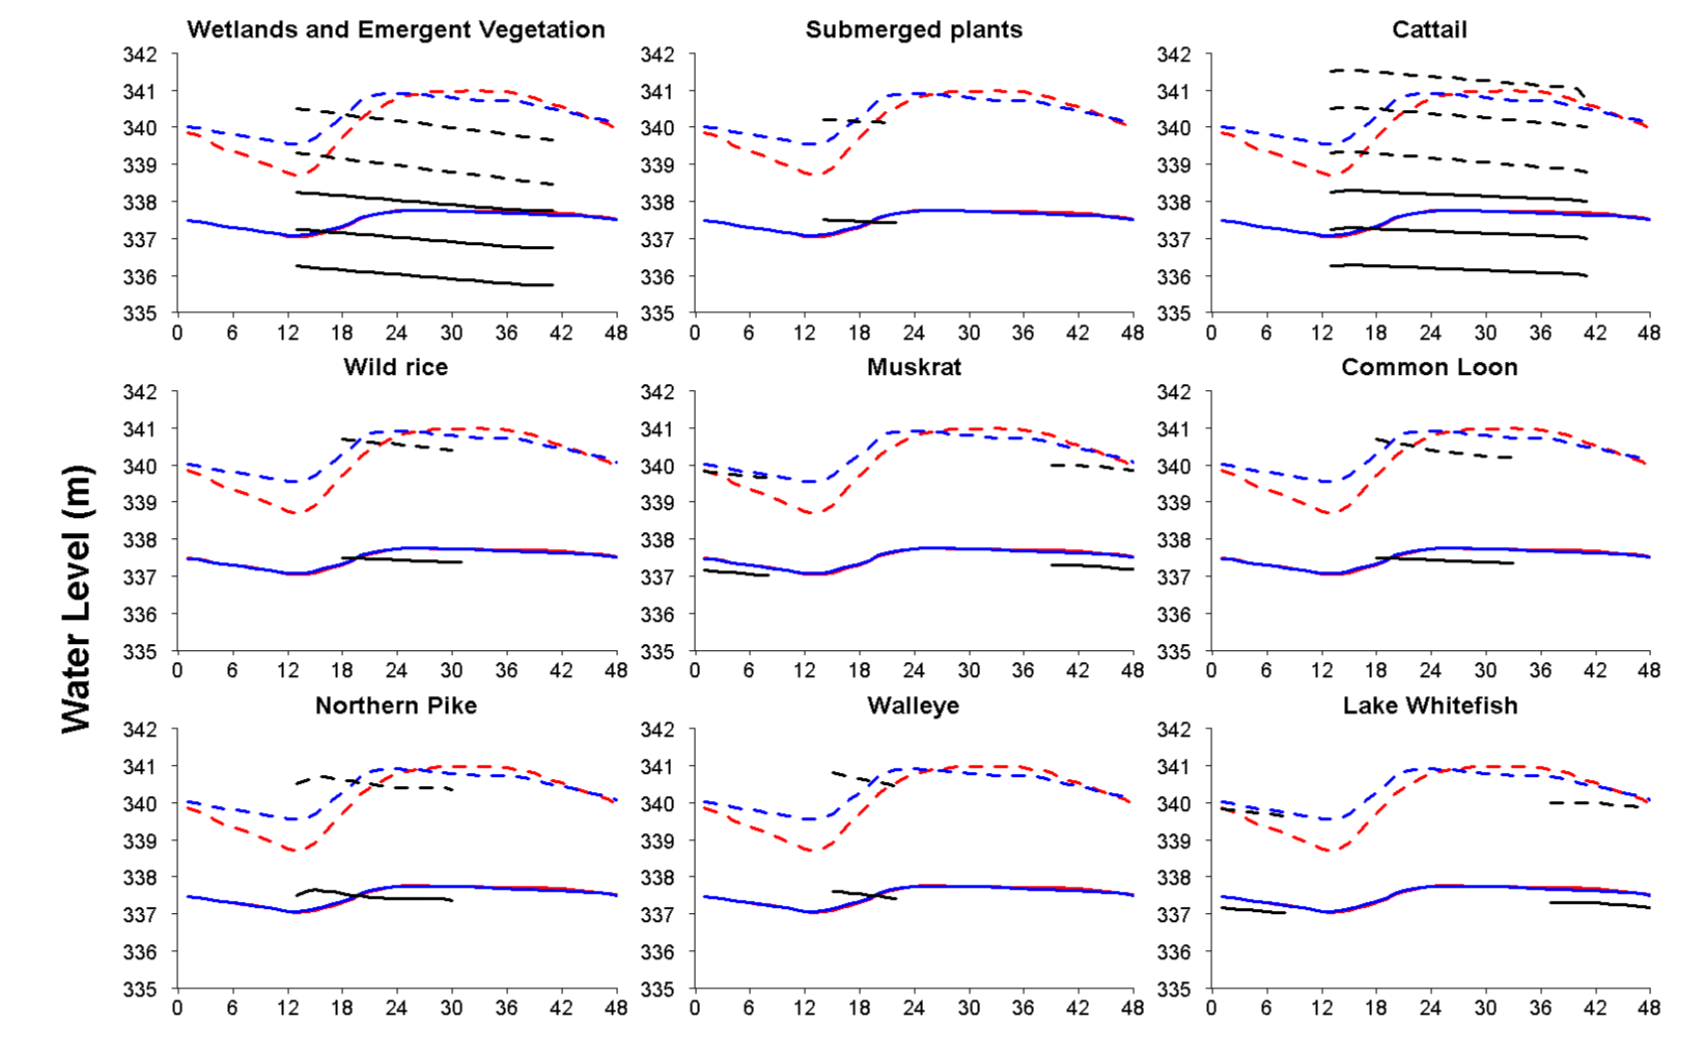
\includegraphics[width=0.8\paperwidth]{MorinRC.png}
\end{center}

\end{frame}

%%%%%%%%%1%%%%%%%%%2%%%%%%%%%3%%%%%%%%%4%%%%%%%%%5%%%%%%%%%6
\begin{frame}{Acknowledgements}
\begin{small}
\begin{itemize}
\item UG Research Assistants:
\begin{multicols}{3}
\begin{itemize}
\item Nicole Mejias
\item Michele Pham
\item Kelly McGarry
\item Usa Wongsanguan
\item Emmy Popovich
\end{itemize}
\end{multicols}
\item \href{http://engineering.nd.edu/profiles/ahamlet/}{Alan Hamlet}, CEEES, Notre Dame
\item \href{http://engineering.nd.edu/profiles/ahamlet/}{Marc Muller}, CEEES, Notre Dame
\item Aaron Thompson, Directorate Environment Canada
\item Jean Morin, Environment and Climate Change Canada
\item RLPOA Research and Technology Committee
\end{itemize}
\end{small}

\end{frame}

%%%%%%%%%1%%%%%%%%%2%%%%%%%%%3%%%%%%%%%4%%%%%%%%%5%%%%%%%%%6
% Section 
%%%%%%%%%1%%%%%%%%%2%%%%%%%%%3%%%%%%%%%4%%%%%%%%%5%%%%%%%%%6

{\usebackgroundtemplate%
	{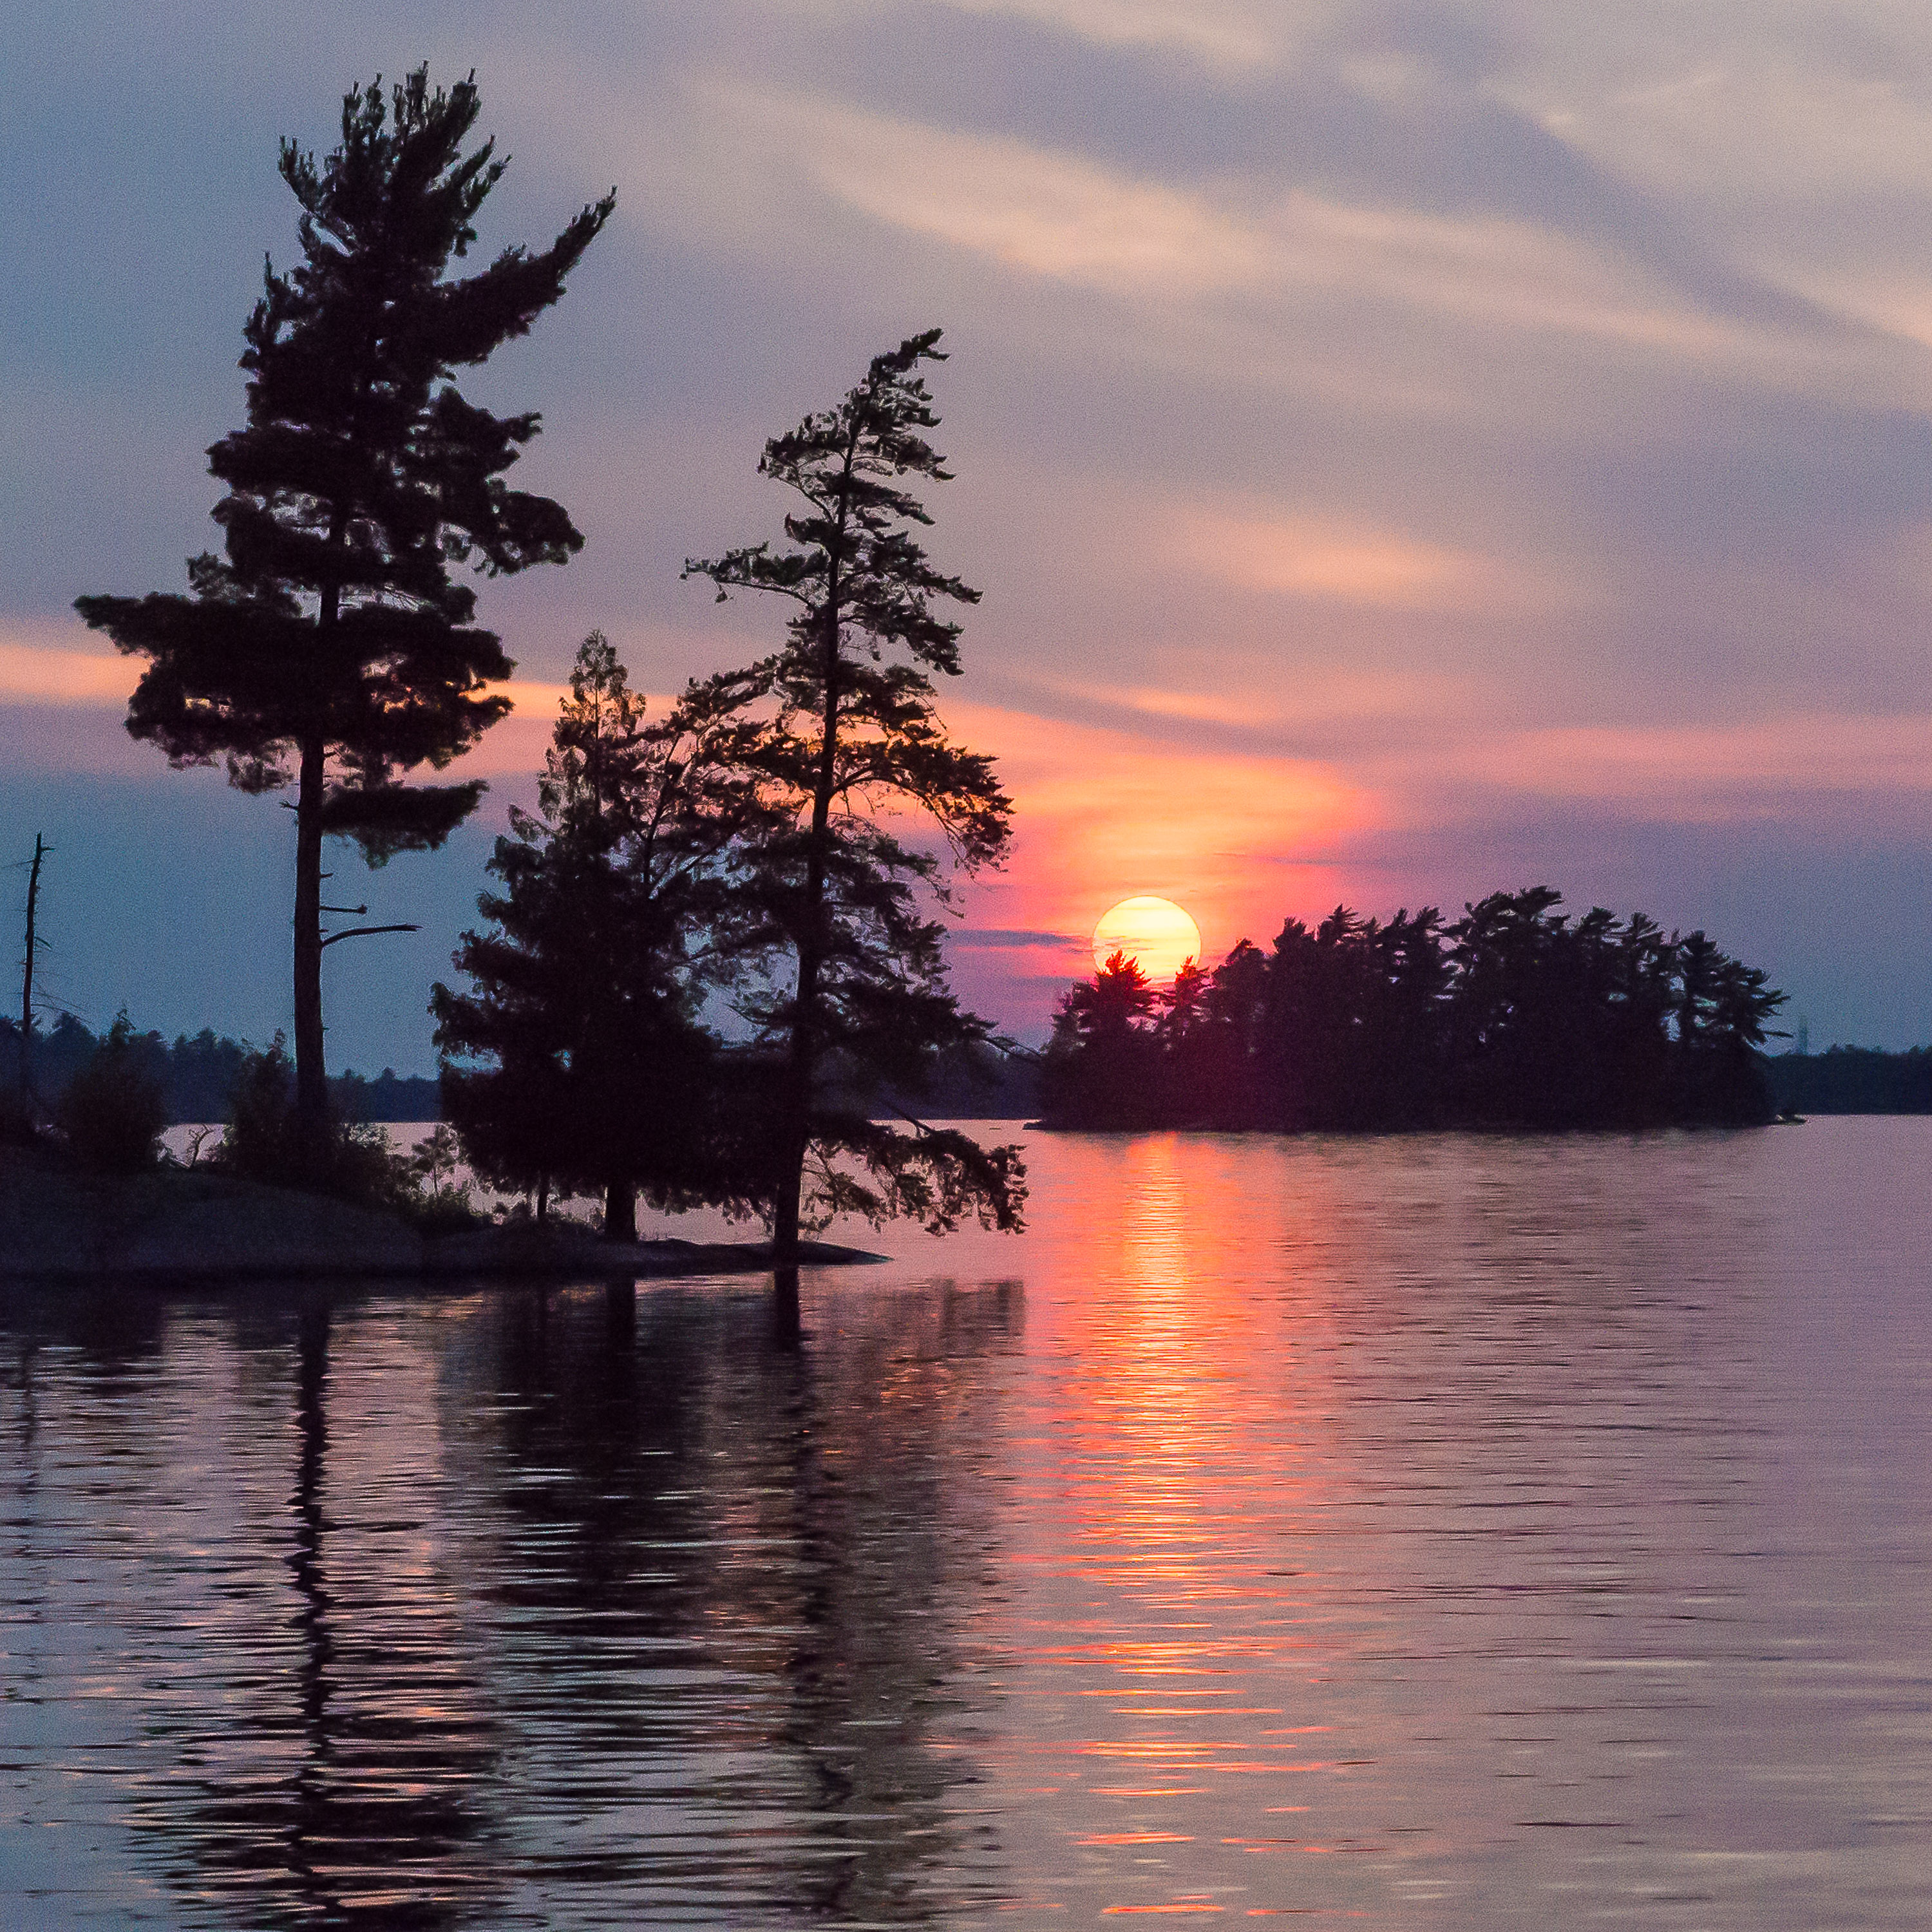
\includegraphics[width=\paperwidth]{FloodedSunset}}
\section{Discussion}
}

%%%%%%%%%1%%%%%%%%%2%%%%%%%%%3%%%%%%%%%4%%%%%%%%%5%%%%%%%%%6
% End of Document
%%%%%%%%%1%%%%%%%%%2%%%%%%%%%3%%%%%%%%%4%%%%%%%%%5%%%%%%%%%6

\end{document}


%%%%%%%%%1%%%%%%%%%2%%%%%%%%%3%%%%%%%%%4%%%%%%%%%5%%%%%%%%%6
\begin{frame}{Global Runoff Data Center - Reporting Stations}

\begin{center}
\includegraphicscopyright[width=0.85\paperwidth]{grdc_stations5.jpg}{Source: GRDC.}
\end{center}
Water information is becoming more scarce.
\end{frame}



